\documentclass[times,sort&compress,3p]{elsarticle}
%\journal{Journal of Multivariate Analysis}
\usepackage[labelfont=bf]{caption}
\renewcommand{\figurename}{Fig.}

\usepackage{amsmath,amsfonts,amssymb,amsthm,booktabs,color,epsfig,graphicx,hyperref,url}

%\usepackage{amsthm}
%\usepackage[demo]{graphicx}
\usepackage{subcaption}
%%%%% PLACE YOUR OWN MACROS HERE %%%%%
\usepackage{verbatim,color,amssymb}
\usepackage{amsmath}					
\usepackage{amsthm}					
%\usepackage{algorithm,algorithmic}
%\usepackage[round]{natbib} %numbers,numbers,
%\usepackage{cite}
\usepackage{setspace}
\usepackage[mathscr]{euscript}
\usepackage{fancyhdr}
\usepackage{enumitem}
\usepackage{graphicx}
\usepackage{geometry}
\usepackage{lineno}
%\usepackage[compact]{titlesec}
\usepackage{listings}
\usepackage{rotating}
%\usepackage{subfig,subfloat}
%\usepackage{multirow}
%\usepackage{lineno}
\usepackage{booktabs}
\def\rot{\rotatebox}
\usepackage{mathtools}
%\usepackage{subfig}
\usepackage{caption}
\usepackage{xr}
\usepackage{xurl}
%\usepackage{kbordermatrix}% http://www.hss.caltech.edu/~kcb/TeX/kbordermatrix.sty
%\renewcommand{\kbldelim}{(}% Left delimiter
%\renewcommand{\kbrdelim}{)}% Right delimiter
%\captionsetup[subfigure]{labelformat=parens,
%	labelsep=space,
%	font=small,
%	margin=0em
%}
\usepackage{float}
%\newsubfloat{figure}% Allow sub-figures
\usepackage{tikz}
\usetikzlibrary{arrows,chains,backgrounds,fit}
\usepackage{multirow}
\usepackage{lineno}

%\def\pdfshellescape{1}

% \setlength{\textheight}{9in}
% \setlength{\textwidth}{6in}
% \setlength{\topmargin}{-36pt}
% \setlength{\oddsidemargin}{15pt}
% \setlength{\evensidemargin}{0pt}
% \tolerance=500
% \renewcommand{\baselinestretch}{1.5}


%\usepackage[english]{babel}
%\usepackage[utf8]{inputenc}
%\usepackage{algorithm}
%\usepackage[noend]{algpseudocode}

%%%%%%%%%%%%%%%
% Begin New Definitions  %%
%%%%%%%%%%%%%%%
%------------------------------------------------------------------------


\theoremstyle{plain}% Theorem-like structures provided by amsthm.sty
\newtheorem{theorem}{Theorem}
\newtheorem{exa}{Example}
\newtheorem{rem}{Remark}
\newtheorem{proposition}{Proposition}
\newtheorem{lemma}{Lemma}
\newtheorem{corollary}{Corollary}

\theoremstyle{definition}
\newtheorem{definition}{Definition}
\newtheorem{remark}{Remark}
\newtheorem{example}{Example}
%------------------------------------------------------------------------
%------------------------------------------------------------------------
\def\bzero{{\mathbf 0}}
\newcommand{\uzero}            {\mbox{\boldmath$0$}}
\newcommand{\uone}               {\mbox{\boldmath$1$}}
\def\etal{\emph{et al.}}

\def\nN{\mathbb{N}}
\def\rR{\mathbb{R}}
\def\eE{\mathbb{E}}

\def\L{{\cal L}}
\def\B{{\cal B}}
\def\C{{\cal C}}
\def\D{{\cal D}}
\def\E{{\cal E}}
\def\F{{\cal F}}
\def\G{{\cal G}}
\def\K{{\cal K}}
\def\M{{\cal M}}
\def\N{{\cal N}}
\def\calP{{\cal P}}
\def\S{{\cal S}}
\def\T{{\cal T}}
\def\U{{\cal U}}
\def\W{{\cal W}}
\def\V{{\cal V}}
\def\X{{\cal X}}
\def\Z{{\cal Z}}
\def\Y{{\cal Y}}
\def\sumi{\sum_{i=1}^n}

\def\scrC{{\mathscr{C}}}


\def\diag{\hbox{diag}}
\def\Ind{\hbox{I}}
\def\wh{\widehat}
\def\wt{\widetilde}
%\def\wb{\breve}
\def\AIC{\hbox{AIC}}
\def\BIC{\hbox{BIC}}
\def\diag{\hbox{diag}}
\def\log{\hbox{log}}
\def\bias{\hbox{bias}}
\def\Siuu{\boldSigma_{i,uu}}
\def\whT{\widehat{\Theta}}
\def\var{\hbox{var}}
\def\cov{\hbox{cov}}
\def\corr{\hbox{corr}}
\def\sign{\hbox{sign}}
\def\trace{\hbox{trace}}
\def\naive{\hbox{naive}}
\def\vect{\hbox{vec}}


\def\Beta{\hbox{Beta}}
\def\DE{\hbox{DE}}
\def\Dir{\hbox{Dirch}}
\def\Exp{\hbox{Exp}}
\def\gIGs{\hbox{g-Inv-Gs}}
\def\Ga{\hbox{Ga}}
\def\IGs{\hbox{Inv-Gs}}
\def\IG{\hbox{Inv-Ga}}
\def\IW{\hbox{IW}}
\def\MVN{\hbox{MVN}}
\def\MatMVN{\hbox{Mat-MVN}}
\def\MVL{\hbox{MVL}}
\def\MVT{\hbox{MVT}}
\def\Normal{\hbox{Normal}}
\def\TN{\hbox{TN}}
\def\Unif{\hbox{Unif}}
\def\Mult{\hbox{Mult}}
\def\Wish{\hbox{W}}


\def\wt{\widetilde}
\def\sumi{\sum_{i=1}^n}
\def\diag{\hbox{diag}}
\def\wh{\widehat}
\def\AIC{\hbox{AIC}}
\def\BIC{\hbox{BIC}}
\def\diag{\hbox{diag}}
\def\log{\hbox{log}}
\def\bias{\hbox{bias}}
\def\Siuu{\boldSigma_{i,uu}}
\def\dfrac#1#2{{\displaystyle{#1\over#2}}}
\def\VS{{\vskip 3mm\noindent}}
\def\refhg{\hangindent=20pt\hangafter=1}
\def\refmark{\par\vskip 2mm\noindent\refhg}
\def\naive{\hbox{naive}}
\def\itemitem{\par\indent \hangindent2\parindent \textindent}
\def\var{\hbox{var}}
\def\cov{\hbox{cov}}
\def\corr{\hbox{corr}}
\def\trace{\hbox{trace}}
\def\refhg{\hangindent=20pt\hangafter=1}
\def\refmark{\par\vskip 2mm\noindent\refhg}
\def\Normal{\hbox{Normal}}
\def\Poisson{\hbox{Poisson}}
\def\Wishart{\hbox{Wishart}}
\def\Invwish{\hbox{Inv-Wishart}}
\def\Beta{\hbox{Beta}}
\def\NiG{\hbox{NiG}}
\def\matF{\hbox{Mat-F}}



\def\ANNALS{{\it Annals of Statistics}}
\def\ANNALSP{{\it Annals of Probability}}
\def\ANNALSMS{{\it Annals of Mathematical Statistics}}
\def\ANNALSAS{{\it Annals of Applied Statistics}}
\def\ANNALSISM{{\it Annals of the Institute of Statistical Mathematics}}
\def\AJE{{\it American Journal of Epidemiology}}
\def\ANIPS{{\it Advances in Neural Information Processing Systems}}
\def\APLS{{\it Applied Statistics}}
\def\BA{{\it Bayesian Analysis}}
\def\BRNL{{\it Bernoulli}}
\def\BIOK{{\it Biometrika}}
\def\BIOS{{\it Biostatistics}}
\def\BMCS{{\it Biometrics}}
\def\BMCMIDM{{\it BMC Medical Informatics and Decision Making}}
\def\BIOINF{{\it Bioinformatics}}
\def\CANADAJS{{\it Canadian Journal of Statistics}}
\def\CG{{\it Current Genomics}}
\def\CDA{{\it Computational Statistics \& Data Analysis}}
\def\COMMS{{\it Communications in Statistics, Series A}}
\def\COMMS{{\it Communications in Statistics, Theory \& Methods}}
\def\COMMSS{{\it Communications in Statistics - Simulation}}
\def\COMMSSC{{\it Communications in Statistics - Simulation and Computation}}
\def\EJS{{\it Electronic Journal of Statistics}}
\def\ECMK{{\it Econometrica}}
\def\ECTH{{\it Econometric Theory}}
\def\GENEP{{\it Genetic Epidemiology}}
\def\JASA{{\it Journal of the American Statistical Association}}
\def\JRSSB{{\it Journal of the Royal Statistical Society, Series B}}
\def\JRSSC{{\it Journal of the Royal Statistical Society, Series C}}
\def\JQT{{\it Journal of Quality Technology}}
\def\JCGS{{\it Journal of Computational and Graphical Statistics}}
\def\JCB{{\it Journal of Computational Biology}}
\def\JAMA{{\it Journal of the American Medical Association}}
\def\JNUTR{{\it Journal of Nutrition}}
\def\JABES{{\it Journal of Agricultural, Biological and Environmental Statistics}}
\def\JBES{{\it Journal of Business and Economic Statistics}}
\def\JSPI{{\it Journal of Statistical Planning \& Inference}}
\def\JMA{{\it Journal of Multivariate Analysis}}
\def\JNS{{\it Journal of Nonparametric Statistics}}
\def\JSS{{\it Journal of Statistical Software}}
\def\JECM{{\it Journal of Econometrics}}
\def\IEEE{{\it IEEE}}
\def\IEEESPL{{\it IEEE Signal Processing Letters}}
\def\IEEETIT{{\it IEEE Transactions on Information Theory}}
\def\LETTERS{{\it Letters in Probability and Statistics}}
\def\ML{{\it Machine Learning}}
\def\P_25_ICML{{\it Proceedings of the 25th international conference on Machine learning}}
\def\PLoSCB{{\it PloS Computational Biology}}
\def\STIM{{\it Statistics in Medicine}}
\def\SCAN{{\it Scandinavian Journal of Statistics}}
\def\SMMR{{\it Statistical Methods in Medical Research}}
\def\SNKH{{\it Sankhy\={a}: The Indian Journal of Statistics}}
\def\STIM{{\it Statistics in Medicine}}
\def\STATMED{{\it Statistics in Medicine}}
\def\STATSCI{{\it Statistical Science}}
\def\SSNC{{\it Statistica Sinica}}
\def\SaC{{\it Statistics and Computing}}
\def\STATSCI{{\it Statistical Science}}
\def\TECH{{\it Technometrics}}


\def\dfrac#1#2{{\displaystyle{#1\over#2}}}
\def\VS{{\vskip 3mm\noindent}}
\def\refhg{\hangindent=20pt\hangafter=1}
\def\refmark{\par\vskip 2mm\noindent\refhg}
\def\itemitem{\par\indent \hangindent2\parindent \textindent}
\def\refhg{\hangindent=20pt\hangafter=1}
\def\refmark{\par\vskip 2mm\noindent\refhg}
\def\povr{\buildrel p\over\longrightarrow}
\def\ccdot{{\bullet}}
\def\bse{\begin{eqnarray*}}
	\def\ese{\end{eqnarray*}}
\def\be{\begin{eqnarray}}
\def\ee{\end{eqnarray}}
\def\bq{\begin{equation}}
\def\eq{\end{equation}}
\def\pr{\hbox{pr}}
\def\wh{\widehat}


\def\boldalpha{{\mbox{\boldmath $\alpha$}}}
\def\boldAlpha{{\mbox{\boldmath $\Alpha$}}}
\def\boldbeta{{\mbox{\boldmath $\beta$}}}
\def\boldBeta{{\mbox{\boldmath $\beta$}}}
\def\bolddelta{{\mbox{\boldmath $\delta$}}}
\def\boldDelta{{\mbox{\boldmath $\Delta$}}}
\def\boldeta{{\mbox{\boldmath $\eta$}}}
\def\boldEta{{\mbox{\boldmath $\Eta$}}}
\def\boldgamma{{\mbox{\boldmath $\gamma$}}}
\def\boldGamma{{\mbox{\boldmath $\Gamma$}}}
\def\boldlambda{{\mbox{\boldmath $\lambda$}}}
\def\boldLambda{{\mbox{\boldmath $\Lambda$}}}
\def\boldmu{{\mbox{\boldmath $\mu$}}}
\def\boldMu{{\mbox{\boldmath $\Mu$}}}
\def\boldnu{{\mbox{\boldmath $\nu$}}}
\def\boldNu{{\mbox{\boldmath $\Nu$}}}
\def\boldomega{{\mbox{\boldmath $\omega$}}}
\def\boldOmega{{\mbox{\boldmath $\Omega$}}}
\def\boldpsi{{\mbox{\boldmath $\psi$}}}
\def\boldPsi{{\mbox{\boldmath $\Psi$}}}
\def\boldsigma{{\mbox{\boldmath $\sigma$}}}
\def\boldSigma{{\mbox{\boldmath $\Sigma$}}}
\def\boldpi{{\mbox{\boldmath $\pi$}}}
\def\boldPi{{\mbox{\boldmath $\Pi$}}}
\def\boldphi{{\mbox{\boldmath $\phi$}}}
\def\boldepsilon{{\mbox{\boldmath $\epsilon$}}}
\def\boldtheta{{\mbox{\boldmath $\theta$}}}
\def\boldTheta{{\mbox{\boldmath $\Theta$}}}
\def\boldve{{\mbox{\boldmath $\ve$}}}
\def\boldVe{{\mbox{\boldmath $\Epsilon$}}}
\def\boldxi{{\mbox{\boldmath $\xi$}}}
\def\boldXi{{\mbox{\boldmath $\Omega$}}}
\def\boldzeta{{\mbox{\boldmath $\zeta$}}}
\def\boldZeta{{\mbox{\boldmath $\Zeta$}}}
\def\boldvarrho{{\mbox{\boldmath $\varrho$}}}
\def\boldVarrho{{\mbox{\boldmath $\Varrho$}}}
\def\boldtau{{\mbox{\boldmath $\tau$}}}
\def\boldTau{{\mbox{\boldmath $\Tau$}}}
\def\boldrho{{\mbox{\boldmath $\rho$}}}
\def\boldRho{{\mbox{\boldmath $\Rho$}}}
\def\boldvarsigma{{\mbox{\boldmath $\varsigma$}}}

\def\trans{^{\rm T}}
\def\myalpha{{\cal A}}
\def\th{^{th}}
\def\bone{{\mathbf 1}}

\def\b1e{{\mathbf e}}
\def\bA{{\mathbf A}}
\def\ba{{\mathbf a}}
\def\bB{{\mathbf B}}
\def\bb{{\mathbf b}}
\def\bc{{\mathbf c}}
\def\bC{{\mathbf C}}
\def\bd{{\mathbf d}}
\def\bD{{\mathbf D}}
\def\bG{{\mathbf G}}
\def\bI{{\mathbf I}}
\def\bk{{\mathbf k}}
\def\bK{{\mathbf K}}
\def\bM{{\mathbf M}}
\def\bp{{\mathbf p}}
\def\bP{{\mathbf P}}
\def\bs{{\mathbf s}}
\def\bS{{\mathbf S}}
\def\bT{{\mathbf T}}
\def\bt{{\mathbf t}}
\def\bu{{\mathbf u}}
\def\bU{{\mathbf U}}
\def\bq{{\mathbf q}}
\def\bQ{{\mathbf Q}}
\def\bV{{\mathbf V}}
\def\bw{{\mathbf w}}
\def\bW{{\mathbf W}}
\def\bx{{\mathbf x}}
\def\bX{{\mathbf X}}
\def\by{{\mathbf y}}
\def\bY{{\mathbf Y}}
\def\bz{{\mathbf z}}
\def\bZ{{\mathbf Z}}
\def\bS{{\mathbf S}}
\def\bzero{{\mathbf 0}}

\def\whT{\widehat{\Theta}}
\def\te{\widetilde{e}}
\def\te{\widetilde{\epsilon}}
\def\tp{\widetilde{p}}
\def\tv{\widetilde{v}}
\def\tmu{\widetilde{\mu}}
\def\tsigma{\widetilde{\sigma}}

\newcommand{\etam}{\mbox{\boldmath $\eta$}}
\newcommand{\bmu}{\mbox{\boldmath $\mu$}}
\newcommand{\bDelta}{\mbox{\boldmath $\Delta$}}
\newcommand{\bphi}{\mbox{\boldmath $\phi$}}
\newcommand{\bpi}{\mbox{\boldmath $\pi$}}
\newcommand{\bPi}{\mbox{\boldmath $\Pi$}}
\newcommand{\bxi}{\mbox{\boldmath $\xi$}}
\newcommand{\bepsilon}{\mbox{\boldmath $\epsilon$}}
\newcommand{\btheta}{\mbox{\boldmath $\theta$}}
\newcommand{\bbeta}{\mbox{\boldmath $\beta$}}
\newcommand{\bgamma}{\mbox{\boldmath $\gamma_{j}$}}
\newcommand{\bzeta}{\mbox{\boldmath $\zeta$}}
\newcommand{\bsigma}{\mbox{\boldmath $\sigma$}}
\newcommand{\bSigma}{\mbox{\boldmath $\Sigma$}}
\newcommand{\balpha}{\mbox{\boldmath $\alpha$}}
\newcommand{\bomega}{\mbox{\boldmath $\omega$}}
\newcommand{\blambda}{\mbox{\boldmath $\lambda$}}
\newcommand{\bLambda}{\mbox{\boldmath $\Lambda$}}
\newcommand{\bOmega}{\mbox{\boldmath $\Omega$}}
\newcommand{\bPsi}{\mbox{\boldmath $\Psi$}}
\newcommand{\bpsi}{\mbox{\boldmath $\psi$}}
\newcommand{\bGamma}{\mbox{\boldmath $\Gamma$}}
\newcommand{\btau}{\mbox{\boldmath $\tau$}}

\newcommand{\abs}[1]{\left\vert#1\right\vert}
\newcommand{\norm}[1]{\left\Vert#1\right\Vert}

\newcommand{\uA}       {\mbox{\boldmath$A$}}
\newcommand{\ua}       {\mbox{\boldmath$a$}}
\newcommand{\uB}       {\mbox{\boldmath$B$}}
\newcommand{\ub}       {\mbox{\boldmath$b$}}
\newcommand{\uC}       {\mbox{\boldmath$C$}}
\newcommand{\uc}       {\mbox{\boldmath$c$}}
\newcommand{\uD}       {\mbox{\boldmath$D$}}
\newcommand{\ud}       {\mbox{\boldmath$d$}}
\newcommand{\uE}       {\mbox{\boldmath$E$}}
\newcommand{\ue}       {\mbox{\boldmath$e$}}
\newcommand{\uF}       {\mbox{\boldmath$F$}}
\newcommand{\uf}       {\mbox{\boldmath$f$}}
\newcommand{\uG}       {\mbox{\boldmath$G$}}
\newcommand{\ug}       {\mbox{\boldmath$g$}}

%\newcommand{\uG}       {\mbox{\boldmath$G$}}

%\newcommand{\ug}       {\mbox{\boldmath$g$}}
\newcommand{\uH}       {\mbox{\boldmath$H$}}
\newcommand{\uh}       {\mbox{\boldmath$h$}}
\newcommand{\uI}       {\mbox{\boldmath$I$}}
\newcommand{\ui}       {\mbox{\boldmath$i$}}
\newcommand{\uJ}       {\mbox{\boldmath$J$}}
\newcommand{\uj}       {\mbox{\boldmath$j$}}
\newcommand{\uK}       {\mbox{\boldmath$K$}}
\newcommand{\uk}       {\mbox{\boldmath$k$}}
\newcommand{\uL}       {\mbox{\boldmath$L$}}
\newcommand{\ul}       {\mbox{\boldmath$l$}}
\newcommand{\uM}       {\mbox{\boldmath$M$}}
\newcommand{\um}       {\mbox{\boldmath$m$}}
\newcommand{\uN}       {\mbox{\boldmath$N$}}
\newcommand{\un}       {\mbox{\boldmath$n$}}
\newcommand{\uO}       {\mbox{\boldmath$O$}}
%\newcommand{\uo}       {\mbox{\boldmath$o$}}
\newcommand{\uP}       {\mbox{\boldmath$P$}}
\newcommand{\up}       {\mbox{\boldmath$p$}}
\newcommand{\uQ}       {\mbox{\boldmath$Q$}}
\newcommand{\uq}       {\mbox{\boldmath$q$}}
\newcommand{\uR}       {\mbox{\boldmath$R$}}
\newcommand{\ur}       {\mbox{\boldmath$r$}}
\newcommand{\uS}       {\mbox{\boldmath$S$}}
\newcommand{\us}       {\mbox{\boldmath$s$}}
\newcommand{\uT}       {\mbox{\boldmath$T$}}
\newcommand{\ut}       {\mbox{\boldmath$t$}}
\newcommand{\uU}       {\mbox{\boldmath$U$}}
\newcommand{\uu}       {\mbox{\boldmath$u$}}
\newcommand{\uV}       {\mbox{\boldmath$V$}}
\newcommand{\uv}       {\mbox{\boldmath$v$}}
\newcommand{\uW}       {\mbox{\boldmath$W$}}
\newcommand{\uw}       {\mbox{\boldmath$w$}}
\newcommand{\uX}       {\mbox{\boldmath$X$}}
\newcommand{\ux}       {\mbox{\boldmath$x$}}
\newcommand{\uY}       {\mbox{\boldmath$Y$}}
\newcommand{\uy}       {\mbox{\boldmath$y$}}
\newcommand{\uZ}       {\mbox{\boldmath$Z$}}
\newcommand{\uz}       {\mbox{\boldmath$z$}}

%%%%%%%%%%%%%%%%%%%%%%%%%%%%%%%%%%%%%%%%%%%%%%%%%%%%%%%%%%%%%%%%%%%%%
\newcommand{\ualpha}            {\mbox{\boldmath$\alpha$}}
\newcommand{\ubeta}             {\mbox{\boldmath$\beta$}}
\newcommand{\ugamma}            {\mbox{\boldmath$\gamma$}}
\newcommand{\udelta}            {\mbox{\boldmath$\delta$}}
\newcommand{\uepsilon}          {\mbox{\boldmath$\epsilon$}}
\newcommand{\uvarepsilon}       {\mbox{\boldmath$\varepsilon$}}
\newcommand{\uzeta}             {\mbox{\boldmath$\zeta$}}
\newcommand{\ueta}              {\mbox{\boldmath$\eta$}}
\newcommand{\utheta}            {\mbox{\boldmath$\theta$}}
\newcommand{\uvartheta}         {\mbox{\boldmath$\vartheta$}}
\newcommand{\uiota}             {\mbox{\boldmath$\uiota$}}
\newcommand{\ukappa}            {\mbox{\boldmath$\kappa$}}
\newcommand{\ulambda}           {\mbox{\boldmath$\lambda$}}
\newcommand{\umu}               {\mbox{\boldmath$\mu$}}
\newcommand{\unu}               {\mbox{\boldmath$\nu$}}
\newcommand{\uxi}               {\mbox{\boldmath$\xi$}}
\newcommand{\uo}                {\mbox{\boldmath$\o$}}
\newcommand{\upi}               {\mbox{\boldmath$\pi$}}
\newcommand{\uvarpi}            {\mbox{\boldmath$\varpi$}}
\newcommand{\urho}              {\mbox{\boldmath$\rho$}}
\newcommand{\uvarrho}           {\mbox{\boldmath$\varrho$}}
\newcommand{\usigma}            {\mbox{\boldmath$\sigma$}}
\newcommand{\uvarsigma}         {\mbox{\boldmath$\varsigma$}}
\newcommand{\utau}              {\mbox{\boldmath$\tau$}}
\newcommand{\uupsilon}          {\mbox{\boldmath$\upsilon$}}
\newcommand{\uphi}              {\mbox{\boldmath$\phi$}}
\newcommand{\uvarphi}           {\mbox{\boldmath$\varphi$}}
\newcommand{\uchi}              {\mbox{\boldmath$\chi$}}
\newcommand{\upsi}              {\mbox{\boldmath$\psi$}}
\newcommand{\uomega}            {\mbox{\boldmath$\omega$}}
%%%%%%%%%%%%%%%%%%%%%%%%%%%%%%%%%%%%%%%%%%%%%%%%%%%%%%%%%%%%%%%%%%
\newcommand{\uGamma}            {\mbox{\boldmath$\Gamma$}}
\newcommand{\uDelta}            {\mbox{\boldmath$\Delta$}}
\newcommand{\uTheta}            {\mbox{\boldmath$\Theta$}}
\newcommand{\uLambda}           {\mbox{\boldmath$\Lambda$}}
\newcommand{\uXi}               {\mbox{\boldmath$\Xi$}}
\newcommand{\uPi}                {\mbox{\boldmath$\Pi$}}
\newcommand{\uSigma}            {\mbox{\boldmath$\Sigma$}}
\newcommand{\uUpsilon}          {\mbox{\boldmath$\Upsilon$}}
\newcommand{\uPhi}              {\mbox{\boldmath$\Phi$}}
\newcommand{\uPsi}              {\mbox{\boldmath$\Psi$}}
\newcommand{\uOmega}            {\mbox{\boldmath$\Omega$}}
%%%%%%%%%%%%%%%%%%%%%%%%%%%%%%%%%%%%%%%%%%%%%%%%%%%%%%%%%%%%%%%%%



%------------------------------------------------------------------------
%------------------------------------------------------------------------
\newcommand{\rsz}[1]{\textcolor{red}{#1}}

\linenumbers

\begin{document}

\begin{frontmatter}

\title{An approximate Bayes factor-based high dimensional MANOVA using random projections}

\author[1]{Roger S. Zoh \corref{mycorrespondingauthor}}
\author[2]{Fangzheng Xie}
%\author[2]{Author Two\corref{mycorrespondingauthor}}

\address[1]{Department of Epidemiology \& Biostatistics, Indiana University, Bloomington, IN 47405, USA}
\address[2]{Department of Statistics, Indiana University, Bloomington, IN 47408, USA}
%\address[2]{Address of Author Two in his country's language and rules}

\cortext[mycorrespondingauthor]{Corresponding author. Email address: \url{rszoh@iu.edu}}

\begin{abstract}
High-dimensional mean vector testing problems for two independent groups remain an active research area. When the length of the mean vector exceeds the groups' combined sample sizes, tests based on the Mahalanobis distance are not applicable since they involve the inversion of rank-deficient sample covariance matrices. Most approaches considered in the literature overcome this limitation by imposing a structure on the covariance matrices. Unfortunately, these assumptions are often unrealistic and difficult to justify in practice. 
%One approach often used to circumvent this problem considers a variant of entries based test that assumes a diagonal covariance matrix, potentially ignoring complex dependency between features. Another approach firstestimate a stable estimate of the covariance matrix assuming a sparsity using a penalty term. Unfortunately, the sparsity assumption for the covariance matrix might not hold in some applications.  
We develop a Bayes factor (BF)-based testing procedure for comparing two or more population means in (very) high dimensional settings while making no a priori assumptions about the structure of the large unknown covariance matrices. Our test is based on random projections (RPs), a popular data perturbation technique. RPs are appealing because they are easy to implement and are virtually applicable to any dependent structure between features in the data. Two versions of Bayes factor-based test statistics are considered. As is typical with data perturbation techniques, tests based on a single random projection can be misleading. Thus, our final test statistic is based on an ensemble of Bayes factors corresponding to multiple replications of randomly projected data. Both proposed test statistics are compared in a series of simulations. Finally, they are applied to the analysis of a publicly available single-cell RNA-seq (scRNA-seq) dataset. 
\end{abstract}

\begin{keyword} %alphabetical order
Bayes factor \sep
Bayesian \sep
High dimension \sep
Mean testing \sep
Random projections 
\MSC[2020] Primary 62H12 \sep
Secondary 62F12
\end{keyword}

\end{frontmatter}


\section{Introduction} \label{sec:intro}

This paper deals with the problem of testing the equality of mean vectors of two or more groups. Suppose that we have data related to $G \geq 2$ independent groups. Let vector $\uX_{gi} \in \mathbf{R}^{p}$ of length $p$ denote the observed data for individual $i$ from the $g^{th}$ group with $n_{g}$ individuals. We further assume $E(\uX_{gi}) = \umu_g$.  
Combining the individual vector data in a single matrix, we have $\uX_{g} = (\uX_{g1}, \ldots, \uX_{gn_g})\trans \in \mathcal{R}^{n_g \times p}$. When $G=2$, we formulate the test problem as follows:
$$ H_{0}: \umu_1 = \umu_2\;\;\;\mbox{against}\;\;\;  \umu_1 \neq \umu_2.  $$
Hypothesis testing for equality of mean vector between two groups continues to receive considerable attention in the literature \cite{zhang2019more, chen2019two}. A significant number of tests proposed in the literature centers on a version of Hotelling's $T^2$ statistic defined as
\be
T^{2} = \frac{n_1n_2}{n_1 + n_2}(\overline{\uX}_2 - \overline{\uX}_1)\trans\uS^{-1}_{12} (\overline{\uX}_2 - \overline{\uX}_1), \label{eq:eqT2}
\ee
where $\uS_{12} = \sum^{2}_{g=1}\sum^{n_g}_{i=1}(\uX_{gi} - \overline{\uX}_g)(\uX_{gi} - \overline{\uX}_g)\trans /(n_1+n_2 - 2)$ is the (pooled) sample covariance, and $\overline{\uX}_g = \sum^{n_g}_{i=1}\uX_{gi}/n_g$ ($g = 1,2$) are the sample mean vectors.
Unfortunately, in its original form \eqref{eq:eqT2}, the statistic $T^2$ can quickly become ill-formed since it involves the inversion of a sample covariance matrix that is rank-deficient when the dimension of the vector is close or exceeds the combined sample size (that is, $n_1+n_2-2 < p$). Various approaches exist in the literature to help circumvent these limitations, and they can be framed as regularization approaches. Among these, some approaches ignore dependency between the features or groups of features \textcolor{black}{and assume a diagonal or fully sparse covariance matrix)} \cite{ahmad2014u,bai1996effect,chen2010two,feng2017composite}, and some other approaches can be viewed as \textcolor{black}{not fully sparse} regularization scheme in an attempt to make the sample covariance invertible but \textcolor{black}{not necessarily diagonal}. Two types of regularization schemes \textcolor{black}{not resulting in diagonal covariance matrices} are often applied \cite{hu2020pairwise}. One regularization scheme adopts a ridge or $L1$-type estimator for the sample covariance matrix \cite{chen2011regularized,li2020adaptable}, whereas the other scheme is based on the random projection (RP) scheme, which resembles a data perturbation approach. Random projection approaches work by projecting high-dimensional data to a low-dimensional subspace while minimally distorting the distances between the data vectors. This eliminates the need to invert a rank-deficient sample covariance matrix and, almost entirely, preserves the distance between the data vectors (\cite{johnson84extensionslipschitz}). 

Recently, random matrix approaches in general and random projections, in particular, have emerged as effective (linear or non-linear) data reduction approaches for various statistical tasks, including clustering (\cite{vrahatis2020ensemble,wan2020sharp}), prediction (\cite{Mukhopadhyay2020targeted}), and hypothesis testing \cite{lopes2011more,srivastava2014raptt, zoh2018powerful}. RPs have been proven to be successful for two-group mean tests \cite{lopes2011more, srivastava2014raptt,zoh2018powerful}. However, to the best of our knowledge, RPs have not been used or evaluated for testing means of more than two groups. Given their wide range of applicability and often their marked computation speed advantages induced by leveraging sparse matrices, there is an interest in studying their use in a MANOVA testing problem. The two-sample mean testing problem in high-dimensional settings is a special case of the more general Multivariate Analysis of Variance (MANOVA) problem. However, extending two-group mean testing procedures to testing the means of more than two groups is not trivial because of the multiplicity of pairwise distances to be simultaneously considered \cite{cai2014high}. In addition, a MANOVA test based on the Bayes factor, for example, will require the practitioner to select many parameters a priori. 

More practically,  if we consider $G$ populations of dimension $p$, with mean vectors $\umu_1, \ldots, \umu_{G}$, respectively, the test problem is formulated as
\be
H_{0}:\; \umu_1 = \umu_2 = \ldots =\umu_G\;   \; \mbox{versus} \; \; H_{1}:\;
% \exists \; 
% (l,k) \in \mathcal{P}\; \mbox{s.t} \;  \; 
\umu_l \neq \umu_k\; \mbox{for some }(l, k) \in \mathcal{P},
\label{eq:test1}
\ee
where $\mathcal{P} = \{(l,k): 1 \leq l < k \leq G  \}$.
Work on the more general MANOVA approaches when $p$ exceeds the sample sizes began more than 60 years ago \cite{dempster1958high,dempster1960significance}. In general, the approaches in the literature differ based on the different assumptions made on the covariance matrix. One approach derives the test under the assumption of common covariances across groups \cite{fujikoshi2004asymptotic}. Another approach removes the assumption of common covariances \cite{srivastava2007multivariate}. We note that most MANOVA tests proposed in the literature are frequentist approaches. However, recently, \cite{zoh2018powerful} shows that a Bayes factor-based restricted most powerful Bayesian test has superior power compared to its frequentist counterpart. Bayesian tests differ from their frequentist counterpart in that the decision to reject the null or accept the null is based on the Bayes factor (BF) and a chosen evidence threshold. Briefly, the Bayes factor in favor of the alternative hypothesis $H_1$ against the null hypothesis $H_0$, denoted by $BF_{10}$, is defined as 
$$BF_{10} = \frac{P(\mbox{Data} \mid H_{1})}{P(\mbox{Data} \mid H_{0})} = \frac{\int f_1(\mbox{Data} \mid \boldTheta_1)\pi(\boldTheta_1 \mid H_{1})d\boldTheta_1}{\int f_0(\mbox{Data} \mid \boldTheta_0)\pi(\boldTheta_0 \mid H_{0})d\boldTheta_0}, \label{eq:test1a}$$
where $P(\mbox{Data} \mid H_{i})$ denotes the marginal distribution of the data under $H_i$, $\pi(\boldTheta_i \mid H_{i})$ denotes the prior distribution of the unknown parameter $\boldTheta_i$ specific to $H_i$, and $f_i(\cdot)$ denotes the data likelihood specific to $H_i$, $i = 0,1$. Note that both the parameters and the data likelihood could potentially depend on the hypotheses. Equation~\eqref{eq:test1a} can involve high-dimensional integrals, and the choice of the prior distribution focuses on distribution forms that lead to closed-formed expressions of the Bayes factor.
 
%RP based approaches include versions for both frequentist \cite{lopes2011more,srivastava2014raptt,thulin2014high} and Bayesian \cite{zoh2018powerful} settings. %Recently, there has been a growing effort towards combining these two approaches in the two-group mean testing problem \cite{hu2020pairwise}.

%As seen before the two group mean testing problem continue to be an active research area.
This paper aims to develop a high-dimensional MANOVA test that relies on RPs to achieve dimension reduction and leverages the framework of restricted most powerful Bayesian tests proposed by \cite{GoddardJohnson} to obtain the parameters of the test statistic. \textcolor{black}{Our proposed test offers a unique advantage compared to current methods as it eliminates the need for any apriori assumptions about the high-dimensional unknown population covariance matrices. Additionally, it expands the existing literature on high-dimensional hypothesis tests using Bayes Factors.} %{\color{blue}[Most importantly, I think we should elaborate more on the contributions of our work compared to the existing literature, including our novelty and the advantage of our approach over the other competitors (if there's any).]}

The rest of the paper is structured as follows. In Section~\ref{sec:test}, we derive the Bayes factor-based tests. Section~\ref{sec:theori} provides the theoretical results of these tests and the simulation results. In Section~\ref{sec:Application}, we apply the proposed method to the analysis of an actual data set from single-cell sequencing (scRNA-Seq). We end with some concluding remarks in Section~\ref{sec:conclusion}. 
 
% section~\ref{sec:simul} evaluate empirical properties of the proposed test through a battery of simulation; in section~\ref{sec:Application} we apply the proposed method to the analysis of an actual data set. We end with some concluding remarks in section~\ref{sec:conclusion} and provide theoretical results of our test in section~\ref{sec:theori}.

\section{Bayes factor-based tests} \label{sec:test}
Consider the following data generating model: $\uX_{gi} = \umu_g + \uepsilon_{gi}$, $g = 1, \ldots, G$ and $i=1, \ldots, n_{g}$, where $G$ denotes the number of independent groups under consideration. 
We assume that $G \geq 2$ and $\uepsilon_{gi}$ are independent and identically distributed (i.i.d.) $\MVN_{p}(\bzero, \uSigma)$ random vectors, $g = 1,\ldots,G$, $i = 1,\ldots,n_g$, where $\MVN_{p}(\mathbf{\mu},\uSigma)$ denotes the $p$-dimensional multivariate normal distribution with mean vector $\mathbf{\mu}$ and covariance matrix $\uSigma$. Suppose the following data are observed (independently) for each of the $G$ groups as $\uX_1 = (\uX_{11}, \ldots, \uX_{1n_1})\trans \in \mathbb{R}^{n_1 \times p}, \ldots,  \uX_G  = (\uX_{G1}, \ldots, \uX_{Gn_G})\trans \in \mathbb{R}^{n_G \times p}$, where the data vectors are stacked row-wise for all $n_g$ individuals in group $g$. %For the rest of the paper, we assume that $p >> \sum^{G}_{g=1}n_g$ and that we are in the "large-p-small-n" setting.
%Let's denote $\mathcal{P} = \{(i,j): 1 \leq i < j \leq G \}$ the collection all unique group indices. %A set of sufficient statistics for the data is $\left(\bar{\uX}_1, \bar{\uX}_2, \ldots, \bar{\uX}_G, \uS_{p}\right)$. Note that $\uS_{p}$ is the pooled covariance estimate of $\uSigma$.
\subsection{Two-group mean test}
When $G=2$, we only have $\uX_1$ and $\uX_2$ and, under the data generating model considered above, the minimal sufficient statistics and their respective sampling distributions are 
\begin{align*}
&\bD_{12} = \overline{\uX}_2 - \overline{\uX}_1 \sim \MVN_{p}(\udelta_{12}, \uSigma), \quad \bA_{12} = 
\frac{n_1\overline{\uX}_1 + n_2\overline{\uX}_2}{n_1+n_2} \sim \MVN_{p}(\umu, \uSigma),\\
&(n_1+n_2-2)\uS_{12} = \sum^{2}_{g=1}(n_g - 1)\uS_g \sim \Wish(n_1+n_2-2, \uSigma), 
\end{align*}
where $\uS_g = \sum^{n_g}_{i=1}(\uX_{gi} - \overline{\uX}_g)(\uX_{gi} - \overline{\uX}_g)\trans /(n_g - 1)$ is the sample covariance matrix for group $g$, $\udelta_{12} = \umu_2 - \umu_1$ is the sample mean difference, $\umu = (n_1\umu_1 + n_2\umu_2)/(n_1+n_2)$, and $\Wish_{p}(n_1+n_2-2,\uSigma)$ denotes the Wishart distribution with degree of freedom $n_1+n_2-2 > 0$ and mean $(n_1 + n_2-2)\uSigma$. 
The Bayesian hypothesis for \eqref{eq:test1} can thus be expressed as
\be
H_0:\; \udelta_{12}\; = \; \uzero\;\; \mbox{with prior} \;\; \pi(\udelta_{12}, \umu, \uSigma | \tau, H_{0}) \;  &\mbox{vs.}& \;
 H_1: \; \udelta_{12} \; \neq \; \uzero\;\;\mbox{with prior} \;\; \pi(\udelta_{12}, \umu, \uSigma \mid \tau, H_{1}) .\;\; \label{eq:hyp1} 
 %H_1: \; \exists (i,j) \in \mathcal{P}\;\; \mbox{s.t}\;\; \udelta_{ij} &\sim& \MVN_{p}(\uzero, \uSigma/\tau_{0,ij})\; \text{and}\; \uSigma \propto |\uSigma|^{-(p+1)/2} \; 
\ee
Similar to \cite{zoh2018powerful}, the generic form of the prior we assume is 
\be
\pi(\udelta_{12}, \umu,\uSigma \mid \tau, H_i) &=& \pi(\udelta_{12} \mid \uSigma, \tau, H_{i})\pi(\umu, \uSigma),\;i=0,1 \label{eq:priorE1}
\ee
and we consider the Jeffrey's prior for $\pi(\umu, \uSigma)$ given as $\pi(\umu, \uSigma) \propto |\uSigma|^{-(p+1)/2}$. Under the null $H_0$, $\pi(\udelta_{12}\mid\mathbf{\mu}, \uSigma, H_0) = \delta_{\mathbf{0}}$ is a point mass at $\uzero$ because $\udelta_{12} = \uzero$. Under the alternative $H_1$, we assume $\pi(\udelta_{12} \mid \mathbf{\mu}, \uSigma, \tau, H_1) \sim \MVN_{p}(\uzero, \uSigma/\tau)$, a scaled multivariate Gaussian prior.    
When $p < n_1 +n_2 -2$, the Bayes factor in favor of the alternative to test the hypothesis in ~\eqref{eq:hyp1} is equal to:
\be
BF_{10,[12]} &=& \left(1 + \eta_{12} \right)^{-m/2} \left[\frac{  1 + {m f_{1,2}}/\{(1 + \eta_{12})(n-m-G+1)\}}{ 1 + {m f_{1,2}}/{(n-m-G+1)}  } \right]^{-(n-1)/2}, \label{eq:BF1a}
\ee
where $\eta_{12} = n_{0,12}/\tau$, $f_{1,2}  = \{(n-p-1) n_{0,12}\}/\{(n-2)p\} (\overline{\uX}_2 - \overline{\uX}_1)\trans\uS^{-1}_{12}(\overline{\uX}_2 - \overline{\uX}_1)$, $n = n_1 + n_2$,
%$f_{1,2}  = \frac{N-m-1)}{(N-2)m} n_{0,12} (\overline{\uX}_1 - \overline{\uX}_2)\uR\trans (\uR\trans\uS_{p}\uR)^{-1}\uR\trans(\overline{\uX}_1 - \overline{\uX}_2)$; $N = n_1 + n_2$;
 $ 1/n_{0,12} = 1/n_1 + 1/n_2$, $\overline{\uX}_g$ is the sample mean of group $g$, $g = 1, 2$, and $\uS_{12}$ is the $p \times p$ pooled sample covariance matrix.

The Bayes factor in \eqref{eq:BF1a} is invalid if $p$ approaches or exceeds $n_1 + n_2 - 2$. Recently, a random projection version of the test was proposed \cite{srivastava2014raptt,zoh2018powerful}. Namely, the data is first projected into a lower subspace of dimension, say $m \in \mathbb{Z}^{+}$, chosen smaller than $n_1 + n_2 -2$ (i.e., $m \in (0, n_1 + n_2 - 2))$. Thus, for a given $m \in (0, n_1 + n_2 - 2)$ and a random projection matrix $\uPhi \in \mathbb{R}^{p \times m}$ where $\uPhi\trans\uPhi = \uI_{m}$ ($\uI_{m}$ denote the identity matrix of dimension $m$), the resulting Bayes factor in favor of the alternative for comparing two groups is 
\be
BF_{10,[12]}(\uPhi) &=& \left(1 + \eta_{12} \right)^{-m/2} \left[\frac{  1 + {m f_{1,2}(\uPhi)}/\{(1 + \eta_{12})(n-m-1)\}}{ 1 + {m f_{1,2}(\uPhi)}/{(n-m-1)}  } \right]^{-(n-1)/2}, \label{eq:BF1}
\ee
where $f_{12}$ in ~\eqref{eq:BF1a} is replaced with $f_{12}(\uPhi) = \{(n-m-1)n_{0,12} \}/\{(n-2)m\} (\overline{\uX}_1 - \overline{\uX}_2)\trans\uPhi(\uPhi\trans\uS_{12}\uPhi)^{-1}\uPhi\trans(\overline{\uX}_1 - \overline{\uX}_2)$. 
In a given problem, different values of $m$ and $\tau$ can affect the performance of the proposed Bayes factor \cite{zoh2018powerful}. We discuss their choices later. 

\subsection{Multiple group mean test: pooled covariance matrix} \label{sec:testpl}

To test the (complex) hypothesis in \eqref{eq:test1} when $G > 2$ and $p > \sum^{G}_{g=1}n_g$, we opt for a testing procedure that very closely resembles the test we used for the two-group case, assuming a common covariance matrix across groups. The hypothesis testing problem is reformulated as
\be
H_{0}:
% \; \; \forall \; (l,k) \in \mathcal{P}\; \mbox{s.t.} \; \; 
\udelta_{lk} = \uzero \; \mbox{for all }(l, k)\in\mathcal{P}
\;\mbox{with prior}\; \pi(\umu_{lk},\uSigma)\; \mbox{versus} \; H_{1}:
% \; \exists \; (l,k) \in \mathcal{P}\; \mbox{s.t.} \;  \; 
\udelta_{lk} \neq \uzero \; \mbox{ for some }(l, k)\in\mathcal{P}
\; \mbox{with prior} \; \pi(\udelta_{lk},\umu_{lk},\uSigma | \tau_{lk}),  \label{eq:test2.2}
\ee
where $\udelta_{lk} = \umu_k - \umu_l$. 
Thus, this will require that we perform $G(G-1)/2$ pairwise tests using a pooled covariance matrix estimated from all groups. Since the null hypothesis in ~\eqref{eq:test2.2} is rejected as soon as one of the $G(G-1)/2$ pairwise tests is rejected, we derive the omnibus Bayes factor for testing \eqref{eq:test2.2}, given a projection matrix $\uPhi \in \mathbb{R}^{p \times m}$ when $p > \sum^{G}_{g=1}n_g$ as:
\be
BF_{10,[ij]}(\uPhi) &=& \left(1 + \eta_{ij} \right)^{-m/2} \left[ \frac{  1 + {m f_{ij}(\uPhi)}/\{(1 + \eta_{ij})(n-m-(G-1))\}}{ 1 + {m f_{ij}(\uPhi)}/{(n-m-(G-1))}  } \right]^{-(n-1)/2}, \label{eq:BFmax}
\ee
% \rsz{
%where we replace the $(12)$ subscript with the $(ij)$ subscript and refer to it as the Bayes factor (BF) in favor of the alternative for comparing group $i$ and $j$. Additionally, the $(ij)$ subscript denotes the pair with the highest $f_{lk}$ value,
% }
%{\color{blue}If my understanding is correct, the definition of $BF_{10}^{\star}$ also depends on the pairwise indices $(i, j)$ through the quantity $\eta_{ij}$? } 
% {\color{black}
where $(i, j) = \left\{(l, k) : f_{lk}(\uPhi) = \max(f_{12}(\uPhi), \ldots, f_{(G-1)G}(\uPhi) )  \right\}$ and $f_{ij}
(\uPhi) = \max(f_{12}(\uPhi), f_{13}(\uPhi), \ldots, f_{(G-1)G}(\uPhi) )$, 
%(\uPhi) = \max_{(l, k)\in\mathcal{P}} f_{lk}(\uPhi)$
% }
the maximum over all the pairwise $f_{lk}(\uPhi)$ (data dependent) statistics computed given a random projection $\uPhi$ across all $G(G-1)/2$ pairs. Note that $(i, j)$ here also implicitly depends on the projection matrix $\uPhi$. Here, for every pair $(l,k)\in\mathcal{P}$, we define  
% {\color{blue}
\[
f_{lk}(\uPhi) = \frac{(n-m-(G-1)) n_{0,lk} }{(n-G)m}(\overline{\uX}_l - \overline{\uX}_k)\trans\uPhi(\uPhi\trans\uS\uPhi)^{-1}\uPhi\trans(\overline{\uX}_l - \overline{\uX}_k),
\]where $n = \sum^{G}_{g=1}n_g$, $n_{0,lk} = (1/n_l + 1/n_k)^{-1}$, $m \in (0,  n - G)$, $\eta_{lk} = n_{0,lk}/\tau_{lk}$,
% for each $(l, k)\in\mathcal{P}$; 
$\uS = \sum^{G}_{g=1} (n_g - 1) S_{g}/(n - G)$ is the pooled sample covariance matrix, and $S_{g} = \sum^{n_g}_{i=1} (\uX_{gi} - \overline{\uX}_{g}) (\uX_{gi} - \overline{\uX}_{g})\trans / (n_g -1)$ is the sample covariance matrix for group $g$, $g = 1,\ldots,G$.
% }
%  \textcolor{red}{
 We use $\tau_{lk}$ to denote the scaling factor for the prior covariance matrix under the alternative for comparing groups $l$ and $k$ and allow $\tau_{lk}$ to be different across pairs. We defer the discussion about the choice of $m$ and $\tau_{lk}$ to later. 

It is important to note that under the data generating model \eqref{eq:test2.2} and a chosen project matrix $\uPhi \in \mathbb{R}^{p \times m}$, $f_{lk}(\uPhi) \sim\uF_{m, n - m- (G-1)}$ for all $(l,k) \in \mathcal{P}$ but not independent across $(l, k)\in\calP$ when $H_{0}$ is true, where $\uF_{\nu_1, \nu_2}$ denotes the central F-distribution with $\nu_1$ and $\nu_2$ degrees of freedom. The lack of independence renders the derivation of the null distribution (or quantiles of the null distribution) of $\max\{f_{12}(\uPhi), f_{13}(\uPhi), \ldots, f_{(G-1)G}(\uPhi) \}$ difficult. %We show the plot comparing the simulated null distribution of $f^{max}$ statistics for various group size and equal group sample sizes for various (common) covariance matrices. (We need to insert the plot of null distribution for $f_{1,2}$).

\subsubsection{Ensemble of test} \label{sec:ensemblT}
From a Bayesian standpoint, we decide to be in favor of the alternative if the Bayes factor exceeds a given evidence threshold $\ugamma_{lk}$, for all $(l, k) \in \mathcal{P}$ \cite{kass1995bayes,lee2014bayesian,stefan2019tutorial}. 
The ranges of thresholds for Bayes factors and their interpretation are provided in \cite{kass1995bayes,lee2014bayesian}. We choose to select the evidence thresholds $\ugamma_{lk}$ for our Bayes Factors to parallel frequentist tests \cite{johnson2013uniformly}. We provide a default way to choose the evidence threshold later. A Bayes factor computed based on a single RP matrix $\uPhi$ can be unstable and very sensitive to the choice of the single RP matrix. Instead, we base our final decision on multiple RPs using an ensemble test. Hence, for $N$ randomly chosen RPs matrices, with $N$ sufficiently large, our final test statistic based on the BF in \eqref{eq:BFmax} is defined as
% {\color{red}
\be
\widetilde{\boldpsi}(N) &=& \frac{1}{N}\sum^{N}_{u=1} \bone \left\{ BF_{10, [i_u j_u]}(\uPhi_u) \geq \ugamma_{i_uj_u} \right\}; \label{eq:BFensblPL}
%\widetilde{\boldpsi}^{PR}(N) &=& \frac{1}{N}\sum^{N}_{u=1} \bone\{ BF^{PR}_{B_u}(\uPhi_u) \geq \gamma^{PR}_{B_u}\}  \label{eq:BFensblPR}
\ee
% }
where $(i_u, j_u)$ represents the pair of groups with the highest value for the $u^{th}$ randomly projected version of the original data set, and $\bone\{C\}$ is the indicator function which equals $1$ if $C$ is true and zero otherwise.
%$BF^{*}_{10}$ is a short hand notation for $\text{BF}^{\star}$ or $\text{BF}^{PR}$ depending in the scenario. 
For the test statistics in \eqref{eq:BFensblPL}, large values of $\widetilde{\boldpsi}(N)$ close to one will tend to favor the alternative.
% as they indicate that the Bayes Factors favor the alternative with high frequency. 
Conversely, lower values of these test statistics will instead favor the null hypothesis $H_0$ of no difference in these group mean vectors. Formally, we will make our final decision based on both test statistics using the following rule:
\be
 \left \{
       \begin{array}{llll}
       \mbox{Reject}~ H_{0}, & \mbox{if} ~~ \widetilde{\boldpsi}(N) > \widetilde{\boldpsi}_{0, \alpha};  \\
       \mbox{Accept}~ H_{0}, & \mbox{otherwise}, \label{eq:ensembleTestPl}
       \end{array}
       \right. \;
\ee
where $\alpha \in (0, 0.5)$, $\widetilde{\boldpsi}_{0, \alpha}$ is the  cut-off value for the test statistic $\widetilde{\boldpsi}(N)$. In the frequentist hypothesis testing scenario, $\widetilde{\boldpsi}_{0, \alpha}$ is selected to achieve a given test size or type I error rate $\alpha > 0$, commonly selected to be small, say $\alpha  = 0.01, 0.05$, when $H_0$ is true. In essence, $\widetilde{\boldpsi}_{0, \alpha}$ represents the upper $\alpha$ percentiles of the null distribution of the test statistics in \eqref{eq:ensembleTestPl} and will be selected for a chosen type I error rate $\alpha$ such that the power of our test is comparable to a frequentist test with the same specify type I error rate.  
Unfortunately, the null distribution, distribution of our test statistics when $H_0$ is true and $\udelta_{lk} = \bzero$ for all $(l,k) \in \mathcal{P}$, is difficult to derive analytically. However, under the assumed data generating model \eqref{eq:test2.2}, the null distribution can be easily approximated using a Monte Carlo approach and a chosen covariance matrix $\uSigma$. Additionally, we find that the null distribution of the test statistics is invariant for arbitrary common mean vector and common (unknown) covariance matrix $\uSigma$. Figure~\ref{fig:BFh0} shows empirical evidence that the distribution of the test statistics $\widetilde{\psi}(N)$ is invariant under the null hypothesis of common vector mean and covariance matrix. We show this for the case of $G=3$ and $G=10$ independent groups simulated under six different covariance matrices ranging from no dependencies to complex dependency (we describe the structure of the covariance matrices in detail in the simulation section (Section~\ref{sec:simdesign}).  
\begin{figure}[H]
%\begin{subfigure}%{0.3\textwidth}
  \centering
\subfloat[10 groups (45 pairs) ]{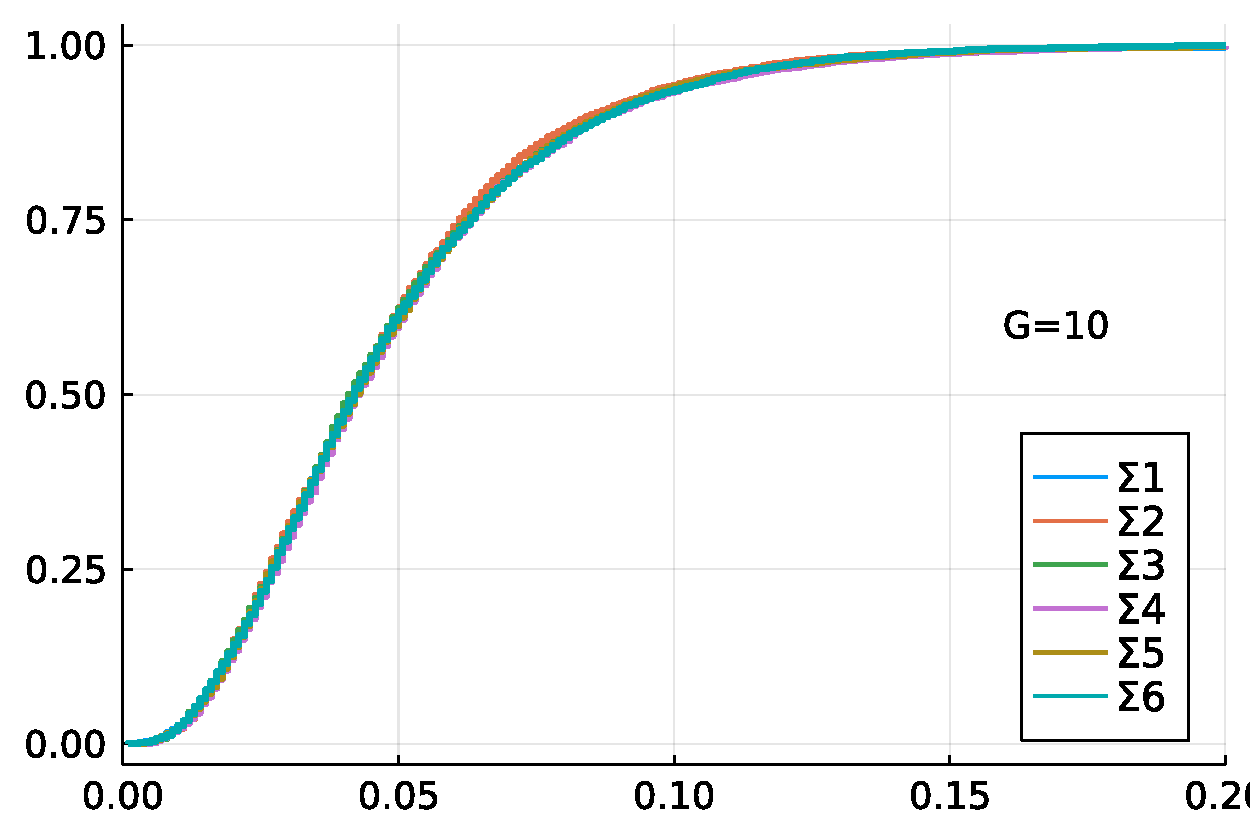
\includegraphics[scale=0.35]{Plots/H0_PR_psi_NullH0_G_10.pdf}}
\subfloat[3 groups (3  pairs )]{ 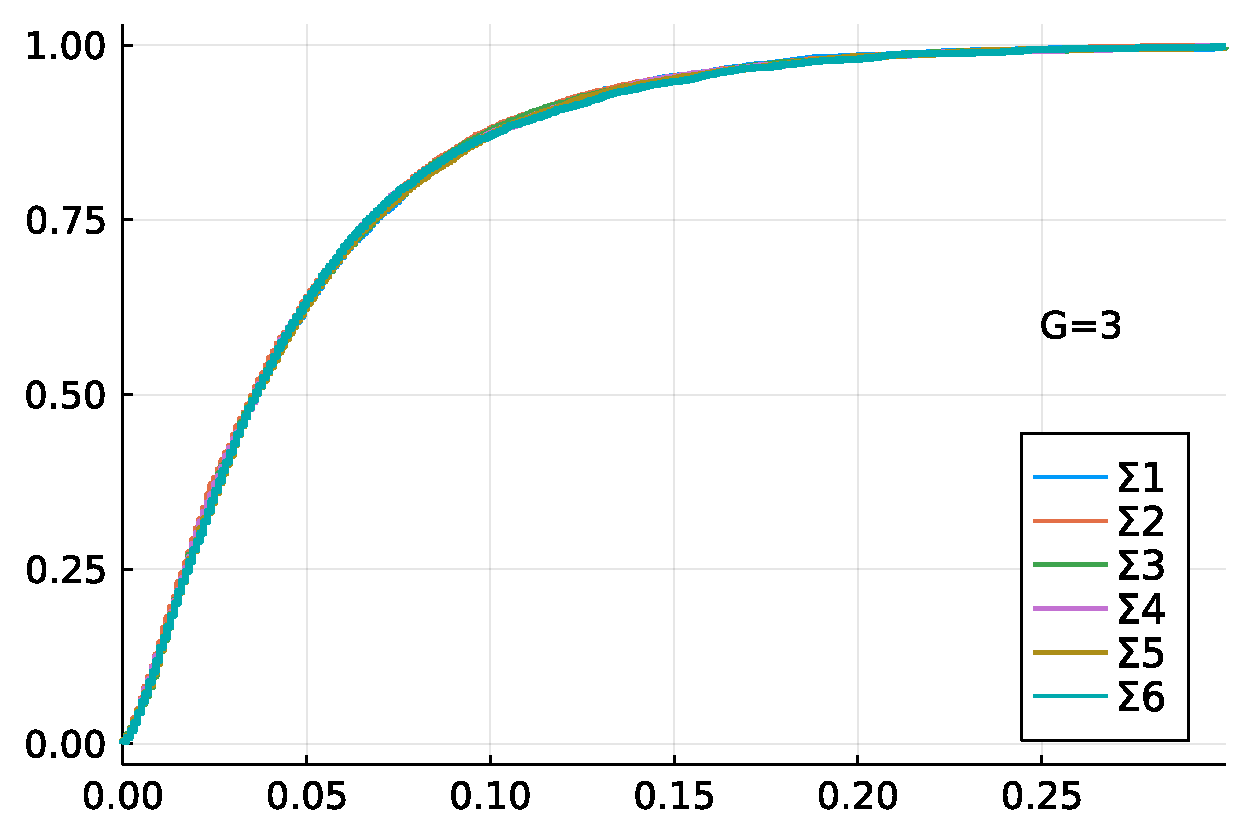
\includegraphics[scale=0.35]{Plots/H0_PR_psi_NullH0_G_3.pdf}}
\caption{Empirical distribution of the test statistics $\widetilde{\psi}(N)$ under the null hypothesis of common mean vector and common covariance matrix across groups. This simulation is based on n = 1000 samples and $N = 1000$ random projections using a dense projection matrix.}
  \label{fig:BFh0}
\end{figure}
  
\subsubsection{Default choices for m, $\tau_{ij}$, $\ugamma_{ij}$} \label{sec:mtaugam}
Our approach requires that we specify some value for the parameters $m$, $\tau_{ij}$, and $\ugamma_{ij}$. Although many different combinations of values would work, it is not clear how they will influence the resulting Bayes factor. Therefore, we consider a more principled way of choosing these parameters to obtain a test statistic that parallels a frequentist test.   
%We provide a default approach to obtaining these parameters $m$, $\tau_{ij}$, and $\gamma^{\star}_{ij}$ needed to compute the test statistics provided in \ref{eq:ensembleTestPl}. Clearly these values can have an impact on the performance of the test. 
Here, we use the idea of restricted most powerful Bayesian test (RMPBT) proposed by \cite{GoddardJohnson,Goddard}. To find the RMPBT, we choose the parameters of the prior distribution under the alternative that maximizes the probability of rejecting the null under all possible parameters of the data generating model in a restricted class of distribution family (here chosen to a scaled multivariate Gaussian). Namely, for a Bayes factor in favor of the alternative computed as in \eqref{eq:BFmax}, we will select $\tau_{ij}$ so that for a given evidence threshold $\ugamma_{ij} > 0$ and any other $\tau^{(2)}_{ij}$ ($\tau^{(2)}_{ij} \neq \tau_{ij}$) associated with a second alternative, we have
$$Pr\left\{BF_{10,[ij]}(\tau_{ij}) \geq  \ugamma_{ij} | H_{1} \right\} \geq Pr\left\{BF_{20,[ij]}(\tau^{(2)}_{ij}) \geq \ugamma_{ij} | H_{2} \right\},$$
for two different choices of the prior parameters under a first alternative $H_1$, represented by $\tau_{ij}$, and a second alternative $H_2$, represented by $\tau^{(2)}_{ij}$). This is equivalent to choosing $\tau_{ij}$ so that $Pr\{f_{ij} > f_{0}(\tau_{ij},\ugamma_{ij})\}$ is maximized, which occurs when $f_{\;0}(\tau_{ij},\ugamma_{ij})$ is minimized over all possible values of $\tau_{ij}$ and $\ugamma_{ij}$. With a little bit of algebra, we can show that 
% $f_{max,\;0}(\tau_{ij},\ugamma_{ij}) =\frac{1+\eta_{ij}}{\eta_{ij}} \left\{ \frac{(N - m -G+1)C_{ij}}{m(1 - C_{ij})} \right\}$, where 
\begin{align*}
    f_{\;0}(\tau_{ij},\ugamma_{ij}) = \frac{1+\eta_{ij}}{\eta_{ij}} \left\{ \frac{(n - m -G+1)C_{ij}}{m(1 - C_{ij})} \right\},\quad
    C_{ij} = \frac{1+\eta_{ij}}{\eta_{ij}}\left[ 1 - \{\ugamma_{ij}(1+\eta_{ij})^{m/2} \}^{-2/(n-1)}  \right],\quad\eta_{ij} = n_{0,ij}/\tau_{ij}
\end{align*}
for the Bayes factor in \eqref{eq:BFmax}. 
Recalling that for all $(l,k) \in \mathcal{P}$, $f_{lk} {\sim} \uF_{m, N - m- (G-1)}$ but not independently across $(l, k)\in\mathcal{P}$ when $H_0$ is true. Then, we can select $f_{0}$ so that our test has the same size as an equivalent frequentist test. Namely, for a significance level $\alpha \in (0, 0.5)$, we will select $f_0(\tau_{ij},\ugamma_{ij}, \alpha)$ so that 
$Pr\{\max_{(l, k)\in\mathcal{P}}f_{lk}(\uPhi) > f_{0}(\tau_{ij},\ugamma_{ij}, \alpha)\} = \alpha$ when $H_{0}$ is true. However, obtaining the upper $\alpha$ percentile of the maximum of dependent $F$-distributed random variables is a difficult task. Using a Monte Carlo step would lead to a significant increase in computation. Under the assumption of common group covariance matrices when $H_0$ is true, we have that: 
$f_{\;0}(\tau_{ij},\ugamma_{ij}, \alpha) \approx \uF_{m, n -m -(G-1)}\{(1 - \alpha)^{1/|\mathcal{P}|}\},$ where $\uF_{a, b}(\theta)$ denotes the upper $\theta$ percentile of an $\uF$ distribution with $a$ and $b$ degrees-of-freedom and $|\mathcal{P}| = G(G-1)/2$. This approximation works well for small values of $\alpha$, which we will tend to be concerned with. We plot the exact and the estimated empirical distribution functions of $\max_{(l, k)\in\mathcal{P}}f_{lk}(\uPhi)$ based on a single random projection along with the case of independence (maximum of independent and identically distributed $F$ random variables) added for comparison (see Figure \ref{fig:fig2}). As we expect, these distributions overlap nicely across all six covariance matrices considered. However, there is a larger discrepancy between the dependent and the independent case in the left tail of the distribution than in the right tail. The difference between these empirical quantiles in the upper tail is very small for higher quantiles.

\begin{figure}%[ht!]
% \begin{tabular}{|l|}
    %\hline
%\begin{subfigure}%{0.3\textwidth}
%\centering
%\centering
    \begin{subfigure}{.4\linewidth}
        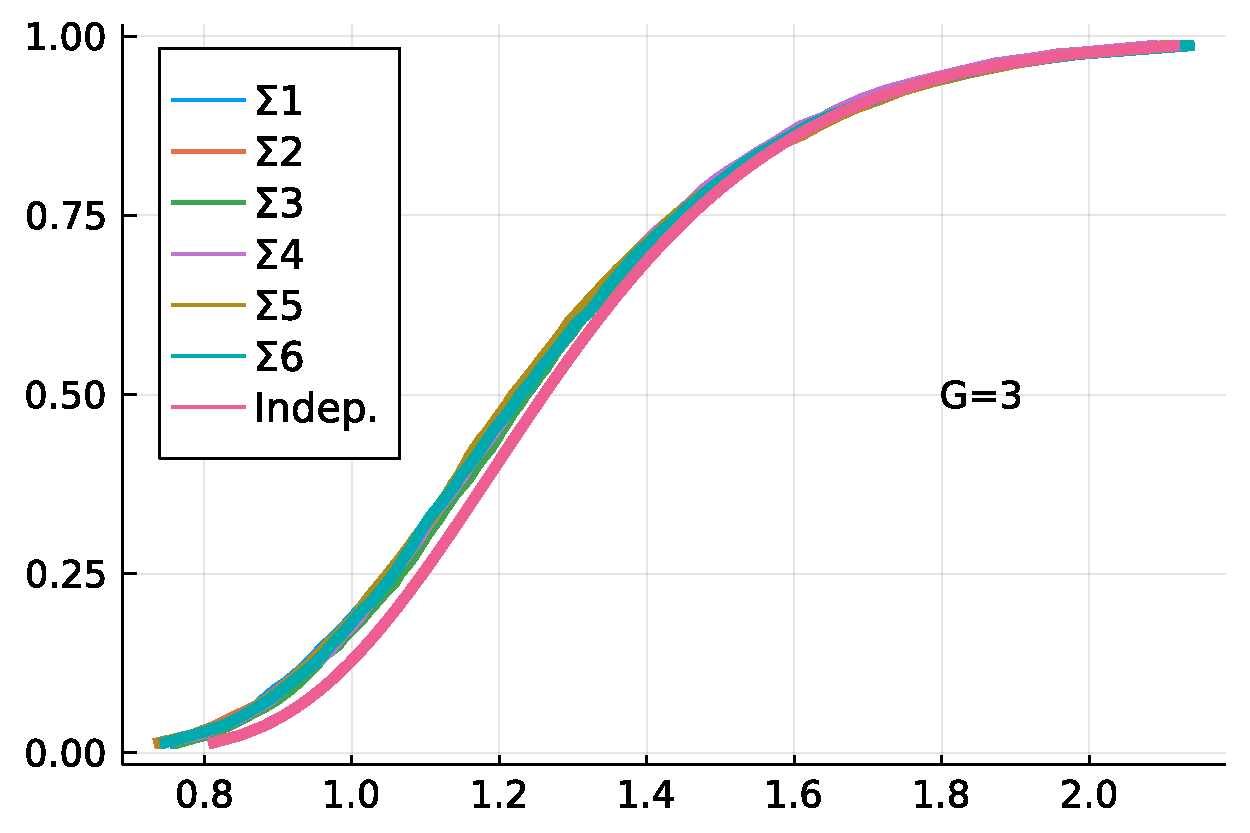
\includegraphics[scale=0.35]{Plots/DistFunc_Plot_of F_statBayF_and_F_indep_G_3.pdf}
        \caption{3 groups (3  pairs )}
    \end{subfigure}
    \hskip2em
    \begin{subfigure}{.4\linewidth}
        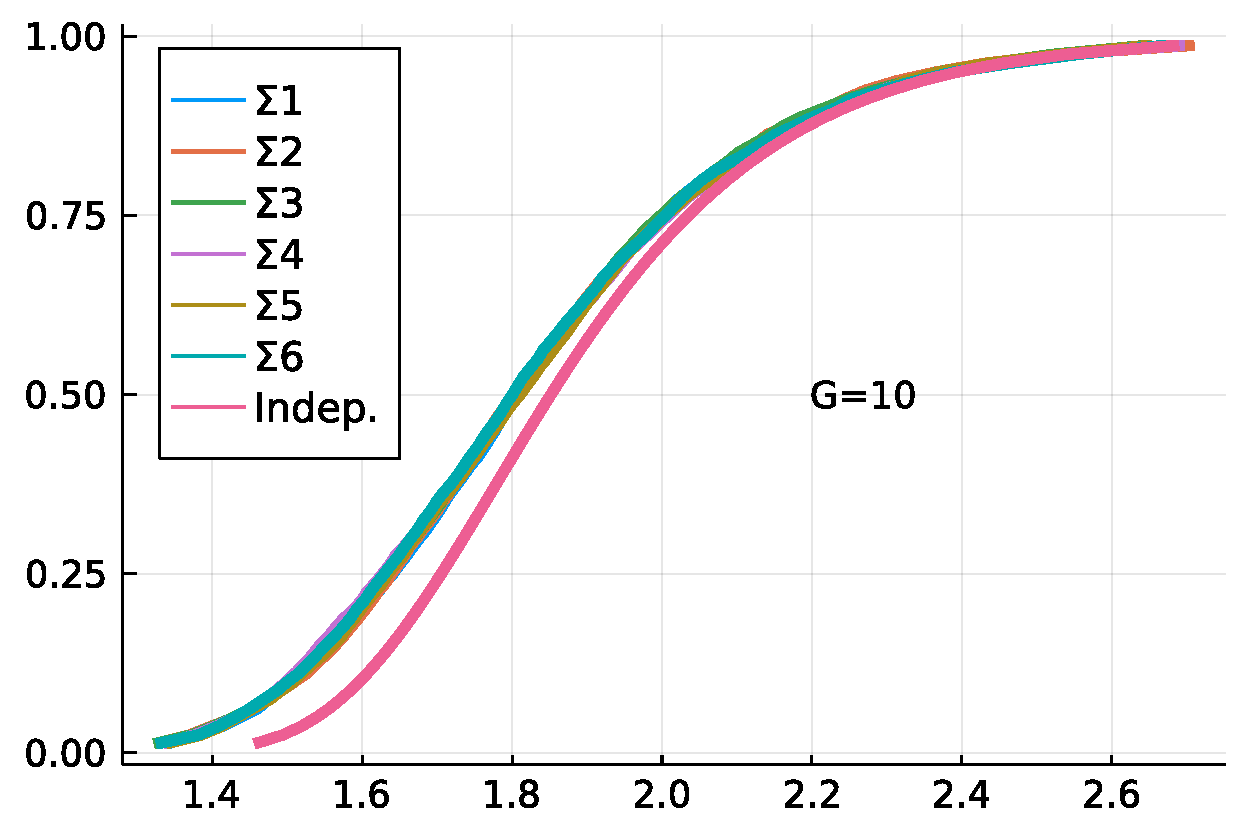
\includegraphics[scale=0.35]{Plots/DistFunc_Plot_of F_statBayF_and_F_indep_G_10.pdf}
        \caption{10 groups (45 pairs)}
    \end{subfigure}
%\subfloat[][10 groups (45 pairs) ]{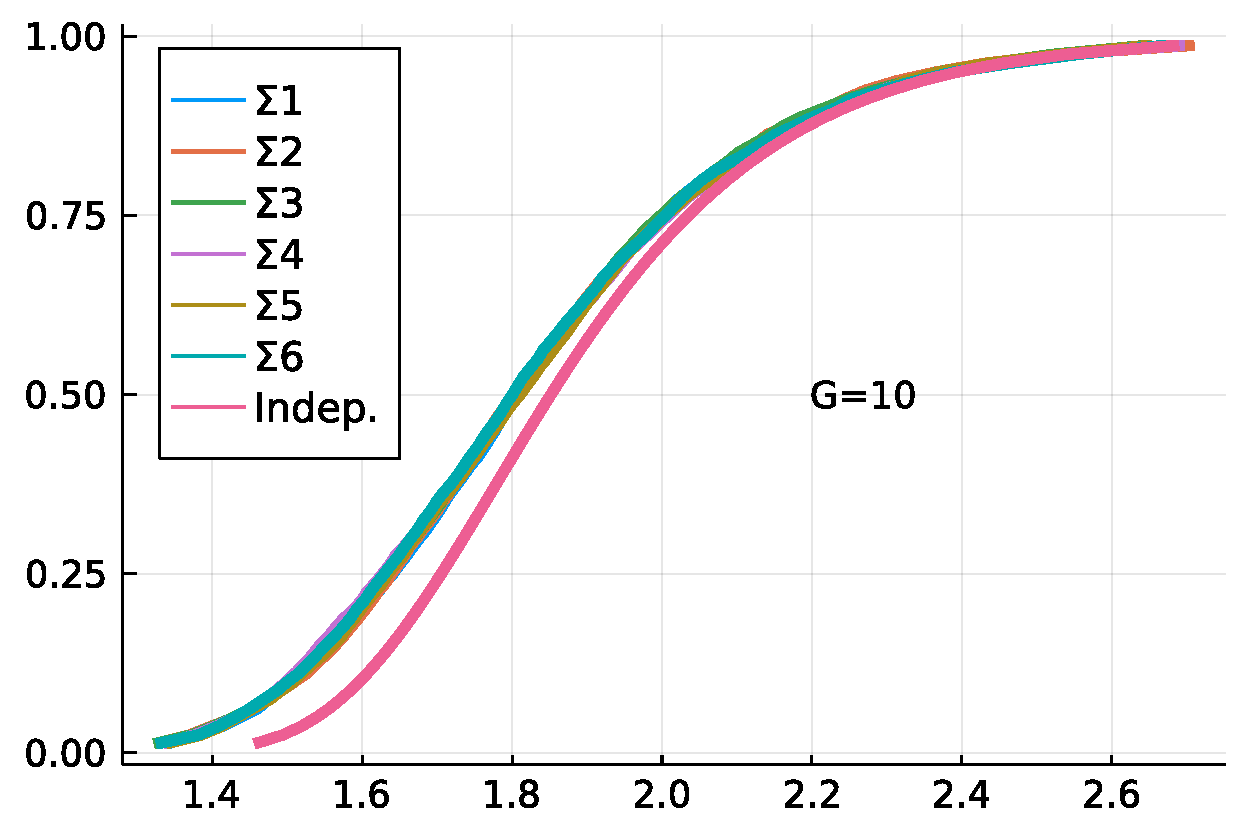
\includegraphics[scale=0.35]{Plots/DistFunc_Plot_of F_statBayF_and_F_indep_G_10.pdf}}
%\subfloat[][3 groups (3  pairs )]{ 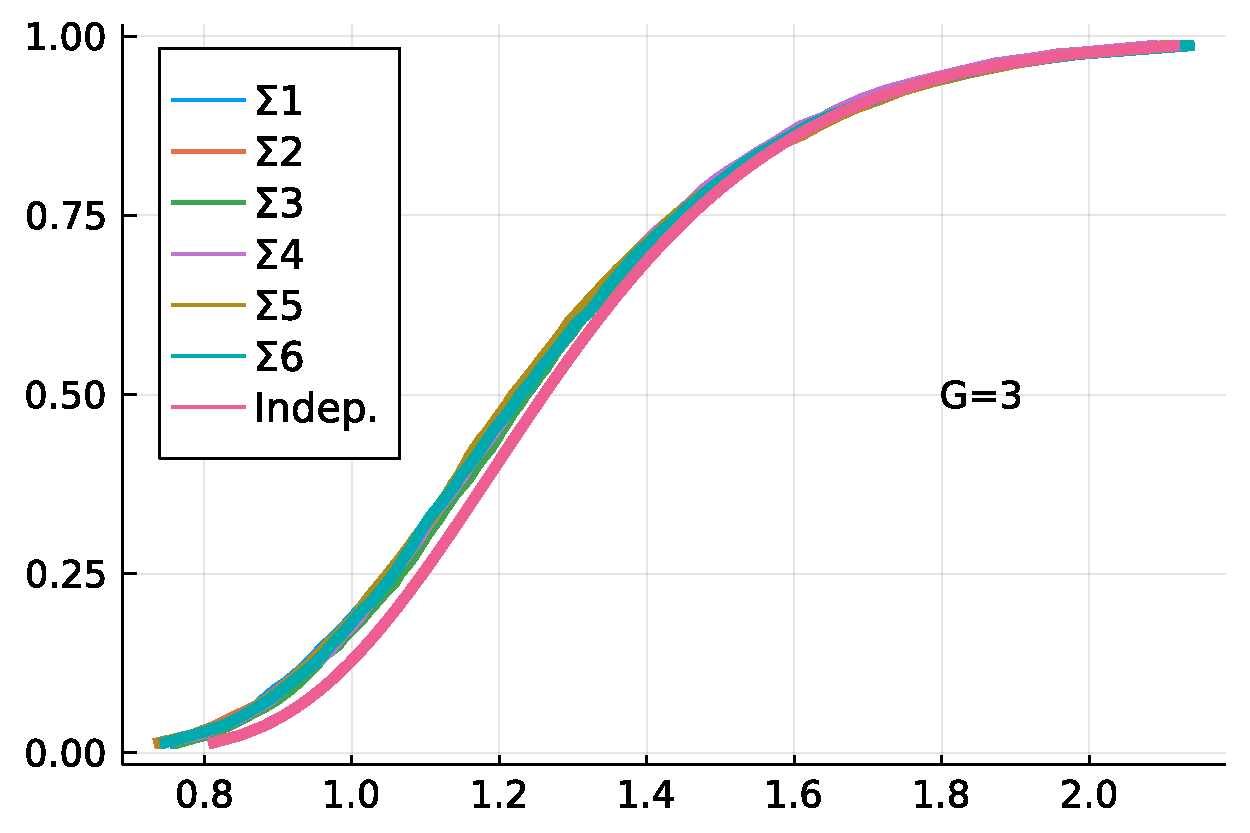
\includegraphics[scale=0.35]{Plots/DistFunc_Plot_of F_statBayF_and_F_indep_G_3.pdf}}
\caption{Plots of the empirical distribution of the maximum of identically but correlated $F$ distributed random variables assuming various covariance structures. We also add the case where these $F$ random variables are independent(Indep.). The sample sizes are identical and set at 50. }
  \label{fig:fig2}
%\label{fig:fmaxquant}
%\end{tabular}
\end{figure}
Finally, for a chosen significance level $\alpha$, we select $m$, the dimension of the random projection space, $\tau_{lk}$, the prior variance scale, and $\ugamma_{lk}$ the evidence threshold comparable as follows, 
%and  which minimizes $\uF_{m, n - m -(G-1)}\{(1 - \alpha)^{1/|\mathcal{P}|}\}$ as
\begin{align*}
&m_n = \underset{u\; \in\; (1, n-G)}{\mathrm{arg\max}}\; \uF_{u, n -u -(G-1)}\{(1 - \alpha)^{1/|\mathcal{P}|}\}, \;
\tau_{lk} = \frac{n_{0,lk}}{\uF_{m_n, n -m_n -(G-1)}\{(1-\alpha)^{1/|\mathcal{P}|}\} - 1},\\
% \mbox{and}\; 
&\ugamma_{lk} = \left\{ 1 + \eta_{lk}\right\}^{-m_n/2}\left\{ 1 - \frac{\eta_{lk}}{1 + \eta_{lk} C_{lk}} \right\}^{-(n -1)/2}, \nonumber
\end{align*}
for all $(l,k) \in \mathcal{P}$, where $C_{lk}$ satisfies ${C_{lk}}/{(1 - C_{lk})} = {\eta_{lk} m_n}/\{(1+ \eta_{lk})(n - m_n -(G-1)\}\uF_{m_n, n -m_n -(G-1)}\{(1 - \alpha)^{1/|\mathcal{P}|}\}.$
The implications of the proposed choices of $m (m_n)$, $\ugamma_{lk}$, and $\eta_{lk}$ on the performance of the test proposed in \eqref{eq:ensembleTestPl} are studied in Section~\ref{sec:theori}. 


\subsection{Multiple group mean test: pairwise pooled covariance matrix} \label{sec:testid}
%The assumption of common covariance across all groups can be too strong in some cases and not supported by the data. We now allow for common pairwise covariance 
\textcolor{black}{Sometimes, the assumption of a shared covariance across all groups may not be well-supported by the available data. We now only allow common pairwise covariance estimates, which are based solely on the two groups being compared. This assumption serves as a working model rather than a data generating model, as assuming pairwise common covariance across all pairs also implies common covariances.}The hypothesis of interest is then expressed as
\be
% H_{0}:\; \; \forall \; (l,k) \in \mathcal{P}\; \mbox{s.t.} \; \; \udelta_{lk} = \uzero\;\; \mbox{and}\;\; \pi(\umu_{lk},\uSigma_{lk})\; \; \mbox{versus} \; \; H_{1}:\; \exists \; (l,k) \in \mathcal{P}\; \mbox{s.t.} \;  \; \udelta_{lk} \neq \uzero\; \; \mbox{and} \; \; \pi(\udelta_{lk},\umu_{lk},\uSigma_{lk} | \tau^{\star}_{lk}), 
H_{0}:\;\udelta_{lk} = \uzero \; \mbox{for all }(l, k)\in\mathcal{P}
\;\mbox{with prior}\; \pi(\umu_{lk},\uSigma_{lk})\; \mbox{versus} \; H_{1}:
% \; \exists \; (l,k) \in \mathcal{P}\; \mbox{s.t.} \;  \; 
\udelta_{lk} \neq \uzero \; \mbox{ for some }(l, k)\in\mathcal{P}
\; \mbox{with prior} \; \pi(\udelta_{lk},\umu_{lk},\uSigma_{lk} | \tau_{lk}^\star), 
\label{eq:test2.3}
\ee
where the covariance matrix is now indexed by the group pair $(l, k)\in\mathcal{P}$ and is allowed to be different across pairs. The priors are as defined above. Subsequently, the Bayes factor in favor of the alternative has the form
\be
BF^{\star}_{10,[ij]}(\uPhi) &=& \left(1 + \eta_{ij} \right)^{-m/2} \left[ \frac{1 + {m f^{\star}_{ij}(\uPhi)}/\{(1 + \eta_{ij})(n_{i}+n_{j}-m-1)\}}{ 1 + {m f^{\star}_{ij}(\uPhi)}/{(n_{i}+n_{j}-m-1)}  } \right]^{-(n_{i}+n_{j}-1)/2}, \label{eq:BFmaxija}
\ee
where $(i, j) = \{(l, k) : f_{lk}^\star(\uPhi) = \max(f_{12}(\uPhi), \ldots, f_{(G-1)G}^\star(\uPhi) )  \}$, $f^{\star}_{ij}(\uPhi) = \max\{f^{\star}_{12}(\uPhi), f^{\star}_{13}(\uPhi), \ldots, f^{\star}_{(G-1)G}(\uPhi)\}$,  
\[
f^{\star}_{lk}(\uPhi) = \frac{(n-m-1)n_{0,lk}}{(n-2)m}  (\overline{\uX}_l - \overline{\uX}_k)\trans\uPhi(\uPhi\trans\uS_{lk}\uPhi)^{-1}\uPhi\trans(\overline{\uX}_l - \overline{\uX}_k),
\]
$\uS_{lk} = ((n_l-1)\uS_{l} + (n_k - 1)\uS_k)/(n_l +n_k -2)$ is the pairwise pooled covariance matrix, $\uS_g = \sum_{i = 1}^{n_g}(\uX_{gi} - \overline{\uX}_g)(\uX_{gi} - \overline{\uX}_g)\trans/(n_g - 1)$ is the sample covariance matrix for group $g$, $g = 1,\ldots,G$, and $1/n_{0,lk} = 1/n_l + 1/n_k$.
Finally, $\eta^{\star}_{lk} = n_{0,lk} /\tau^{\star}_{lk}$, where we allow $\tau^{\star}_{lk}$, the prior scaling factor for $\udelta_{lk}$ under the alternative, to be different across pairs. This allows for additional flexibility in the prior under the alternative.  
Note that for any $ (l,k) \in \mathcal{P}$, $f^{\star}_{lk}{\sim} \uF_{m, n_{l}+n_{k} - m- 1}$ and these distributions are no longer identical, except in the case of same sample sizes across groups, and these random variables are not independently distributed. 

Similar to the test in \eqref{eq:BFensblPL}, the final test statistic for testing hypothesis \eqref{eq:test2.3} is also an ensemble test 
\be
\widetilde{\boldpsi}^{\star}(N) &=& \frac{1}{N}\sum^{N}_{u=1} \bone \left\{ BF^{\star}_{10, [i_u j_u]}(\uPhi_u) \geq \ugamma^{\star}_{i_u j_u} \right\}, \label{eq:BFensblPW}
\ee
where $\ugamma^{\star}_{i_u j_u}$ the evidence threshold. 
Based on a value of the test statistics in \eqref{eq:BFensblPW}, we use the following rule to make a decision
\be
 \left \{
       \begin{array}{llll}
       \mbox{Reject}~ H_{0}, & \mbox{if} ~~ \widetilde{\boldpsi}^{\star}(N) > \widetilde{\boldpsi}^{\star}_{0, \alpha},  \\
       \mbox{Accept}~ H_{0}, & \mbox{otherwise}, \label{eq:ensembleTestPw}
       \end{array}
       \right. \;
\ee
where $\alpha \in (0, 0.5)$, $\widetilde{\boldpsi}^{\star}_{0, \alpha}$ is the cut-off value for the test statistic $\widetilde{\boldpsi}^{\star}(N)$ similarly defined above (see Section~\ref{sec:ensemblT}). Note that for a given value of $\alpha$, $\widetilde{\boldpsi}^{\star}_{0, \alpha}$ can be obtained in the same fashion as described above. Additionally, the choice of the $m$, $\tau^{\star}_{ij}$, and $\ugamma^{\star}_{ij}$ parallels what we discussed in Section~\ref{sec:mtaugam}. We will not discuss these steps in detail here but provide detailed steps in the \textcolor{black}{Supplemental Material}.    

\subsection{Choice of the projection matrix $\uPhi$}
Random projections (RPs), as a data reduction technique, was formalized by the Johnson-Lindenstrauss lemma \cite{johnson84extensionslipschitz}, which shows that vector in high-dimension can effectively be projected into a much lower dimension while minimally distorting their distances. If we denote the RP matrix of dimension $p \times m$ as $\uPhi = (\phi_{rc})$, where $m << p$. The elements $\phi_{rc}$ are then independently simulated, and sparsity or orthogonal structures are subsequently imposed. Various options of RPs have been considered \cite{achlioptas2001database,li2006very,lopes2011more}. We use a dense projection matrix, and a sparse projection matrix similar to the projection matrices used in \cite{srivastava2014raptt,zoh2018powerful}.      

\section{Theoretical justifications and Simulation Results} \label{sec:theori}
We investigate the large sample properties of the proposed tests. 
Here, we adopt a slightly different notation to clarify that the quantities we refer to depend on the sample sizes $n_1, \ldots, n_{G}$. Also, let $n_{\min} = \min\{n_1,\ldots, n_{G}\}$, $n_{\max} = \max\{n_1,\ldots, n_{G}\}$, $n = \sum^{G}_{g=1}n_g$, $n_{ij} = n_i + n_j$, and , $1/n_{0,ij} = 1/n_i + 1/n_j$. %$n_{ij,\min} = \min\{n_{12}, n_{13}, \ldots, n_{(G-1)G} \}$

\subsection{Theoretical Justifications} 
Before proceeding to the theory, several necessary conditions are in order.
\begin{description}
  \item[Assumption 1:] $n_g /\sum_{g=1}^{G}n_g \rightarrow \theta_g \in (0, 1)$ for $g=1,\ldots, G$ as $n_{\min} \rightarrow +\infty$. 
%   {\color{blue}(Are the group sizes required to be asymptotically the same or they can have different limit proportions?)} \rsz{No - I have made the update!}
  \item[Assumption 2:] $G$ is a fixed constant as $n_{\min} \rightarrow \infty$.
 \end{description}
  Roughly speaking, the assumptions above requires that each group occupies a nonvanishing proportion in terms of their sample sizes and the number of groups $G$ is held fixed as $n_{\min}\to\infty$.

\subsubsection{Consistency of test based on the pooled covariance matrix}
Consider the Bayes factor proposed in \eqref{eq:BFmax}. The following theorem shows its large sample behavior for different choices of the $m$, $\tau_{ij}$, and $\ugamma_{ij}$. 
\begin{theorem}\label{Thrm1}
Suppose that $X_{gi} = \umu_g + \uepsilon_{gi}$, where $\uepsilon_{gi} \sim \MVN_{p}(\bzero, \uSigma)$ independently for $g = 1, \ldots, G$ and $i = 1,\ldots,n_g$. Let $m \rightarrow \infty$ with $ \lim_{n_{\min} \rightarrow \infty} m / n =  a \in  (0, 1)$. For a sequence of a projection matrices $\uPhi \in \mathbb{R}^{p \times m}$ as $n_{\min} \rightarrow \infty$, we have:
%Let $p >> n_{\max}$, $G / n_{\min} \rightarrow 0$, and $n_g /\sum_{g=1}^{G}n_g \rightarrow \theta_g \in (0, 1)$ for $g=1,\ldots, G$ as $n_{\min} \rightarrow +\infty$. 
%Given a projection matrix $\uPhi \in \mathbb{R}^{p \times m}$, we have the following: %Suppose $1 \leq m  \leq \min\{n_1, \ldots, n_{G}\}$ and $n_{min} = \min\{n_1, \ldots, n_{G}\}$. Then,  %\sum^{G}_{g=1}n_g$. %Let's $BF_{max} = \max\{BF_{12}, \ldots, BF_{(G-1)G}\}$, where $BF_{ij}$ is the BF based on the group $i$ and $j$ data. As $\min\{n_1, \ldots, n_{G}\} \rightarrow \infty$,
\begin{enumerate}
    \item If $\tau_{ij}$ is a fixed constant, 
    % $\forall (i,j) \in \mathcal{P}$ are pairs, 
    then $\log\left\{BF_{10, [ij]}(\uPhi) \right\} \rightarrow -\infty$ under $H_0$ and $\log\left\{BF_{10, [ij]}(\uPhi) \right\} \rightarrow \infty$ under $H_1$. 
    % {\color{blue}I guess the condition $m/n\to \theta\in (0, 1)$ is required in part (1)? Also, it seems that $\tau_{ij}^{\star}$ should be fixed here?}
    % \rsz{I have made the changes below - we don't need $m/n \rightarrow \theta \in (0,1)$. }
    \item However, if 
    % $1 \leq m_n \leq n - G$ so that $m_n/n \rightarrow \theta \in (0, 1)$
    $n_{0,ij}/\tau_{ij} \rightarrow 0$ such that $n_{0,ij}m/\tau_{ij} \rightarrow \infty$ as $n_{\min} \rightarrow \infty$,  
    %are selected according to our construction in Section~\ref{sec:mtaugam} then: 
    % {\color{red}
   
    \begin{itemize}
        \item[(a)] Under $H_0$, $\log\left\{BF_{10, [ij]}(\uPhi) \right\} = \mathcal{O}_{p}(1)$;
        \item[(b)] 
        % {\color{red} 
        For a sequence of alternatives hypotheses $(H_{1,n})_{n = 1}^\infty$ and projection matrices $\mathbf{\Phi}$ satisfying $\|\mathbf{\Phi}\trans\udelta_{lk}\|_2\to\infty$ and $\|\bSigma\|_2 = O(1)$, then $\log\left\{BF_{10, [ij]}(\uPhi) \right\} \rightarrow \infty$ in probability under $H_{1,n}$. 
        % }
    \end{itemize} 
    % under $H_0$ and  under a sequence of local alternative $H_{1,n}$ as $n_{min} \rightarrow \infty$.
\end{enumerate}
\end{theorem}
The proof of Theorem~\ref{Thrm1} is given in the Appendix.

\subsubsection{Consistency of Bayes factor based on pairwise pooled covariance matrix}
Consider the Bayes factor defined in \eqref{eq:BFmaxija}. 
\begin{theorem}\label{Thrm2}
%Consider the Bayes factor proposed in \eqref{eq:BFmaxija}. We have the following theorem that show its large sample behavior for different choice of the $m$, $\tau_{ij}$, and $\gamma^{\star}_{ij}$. 
%\begin{theorem}\label{Thrm1}
Suppose that $X_{gi} = \umu_g + \uepsilon_{gi}$, where $\uepsilon_{gi} \sim \MVN_{p}(\bzero, \uSigma)$ independently for $g = 1, \ldots, G$ and $i = 1,\ldots,n_g$. Let $m \rightarrow \infty$ with $ \lim_{n_{\min} \rightarrow \infty} m / n =  a \in  (0, 1)$. For a sequence of a projection matrices $\uPhi \in \mathbb{R}^{p \times m}$, and as $n_{\min} \rightarrow \infty$, we have:
 %Suppose $1 \leq m  \leq \min\{n_1, \ldots, n_{G}\}$ and $n_{min} = \min\{n_1, \ldots, n_{G}\}$. Then,  %\sum^{G}_{g=1}n_g$. %Let's $BF_{max} = \max\{BF_{12}, \ldots, BF_{(G-1)G}\}$, where $BF_{ij}$ is the BF based on the group $i$ and $j$ data. As $\min\{n_1, \ldots, n_{G}\} \rightarrow \infty$,
\begin{enumerate}
    \item If $\tau^{\star}_{ij}$ is a fixed constant, 
    % $\forall (i,j) \in \mathcal{P}$ pairs, 
    then $\log(BF^{\star}_{10, [ij]}) \rightarrow -\infty$ under $H_0$ and $\log(BF^{\star}_{10, [ij]}) \rightarrow \infty$ under $H_1$. 
    \item However, if $n_{0,ij}/\tau^{\star}_{ij} \rightarrow 0$ such that $n_{0,ij} m/\tau^{\star}_{ij} \rightarrow \infty$, then
    \begin{itemize}
     \item[(a)]  $\log(BF^{\star}_{10, [ij]}) = \mathcal{O}_{p}(1)$ under $H_0$ as $n_{\min} \rightarrow \infty$ 
     \item[(b)] 
    %  {\color{red}
     For a sequence of alternative hypotheses $(H_{1,n})_{n = 1}^\infty$ and the projection matrix $\mathbf{\Phi}$ satisfying $\|\mathbf{\Phi}\trans\udelta_{lk}\|_2\to\infty$ and $\|\bSigma\|_2 = O(1)$, then $\log(BF^{\star}_{10, [ij]}) \rightarrow \infty$ in probability under $H_{1,n}$. 
    %  }
    \end{itemize}
    %$\log(BF_{ij}) \rightarrow \infty$ under a sequence of local alternative $H_{1,n}$ as $n_{min} \rightarrow \infty$.
\end{enumerate}
\end{theorem}
The proof of Theorem \ref{Thrm2} is very similar to Theorem~\ref{Thrm1} and is omitted here. 
% }
\begin{comment}
\begin{proof}[\textbf{\upshape Proof:}]
\begin{description}
\item[Part(1)]
For $1 < m < \min\{ n_1, \ldots, n_{G} \}$ and $n = n_i + n_j$, we integrate out the parameters usi the conjugate priors to obtain the Bayes factor in favor of the alternative as
\be
BF^{PR}_{10,ij}(\uPhi) &=&\left(1 + \eta_{ij} \right)^{-m/2} \left\{ 1 -  \frac{ m f_{ij} \eta_{ij}/(1 + \eta_{ij}) }{ m f_{ij}  + n_{ij} - m - 1} \right\}^{-(n_{ij}-1)/2} \nonumber,
\ee
where
\bse
f_{ij}  = \frac{n_{ij} - m - 1}{(n_{ij}-2)m} n_{0,ij}(\overline{\uX}_i - \overline{\uX}_j)\trans \uPhi(\uPhi \uS_{ij}\uPhi\trans )^{-1}\uPhi\trans (\overline{\uX}_{i} - \overline{\uX}_{j}).
\ese
where $$ \uS_{ij} = \frac{1}{n_{ij} - 2} \sum_{g=(i,j)}(n_g -1)\uS_{g}\; \text{and} \;\; \uS_g = \frac{1}{n_g - 1}\sum^{n_g}_{l=1}(\uX_lg - \overline{\uX}_{g})(\uX_lg - \overline{\uX}_{g})\trans.$$
Recall that $1/n_{0,ij} = 1/n_i + 1/n_j$, $\eta_{ij} = n_{0,ij}/\tau_{0,ij}$, and $n_{\min} = \min\{n_i, n_j\}$.
Since $\tau_{0,ij}$ is fixed, $\eta_{ij} \rightarrow \infty$ as $n_{\min} \to \infty$.
For a randomly chosen $\uPhi$, under $H_{0}$, $f_{ij}  \sim F_{m, n_{ij}-m-1}$ with $m$ and $n_{ij} - m -1$ degrees of freedom.
Thus, $f_{ij} = O_{p}(1)$ and $f^{max}_{ij} = \max_{ij}\{ f_{ij}\}$ for all $1 \leq i, j \leq G$.
Also, from well-known properties of the $F$ distribution, we have that
\bse
U_{ij} = \frac{m f_{ij}/(n_{ij}-m-1 )}{\{m f_{ij}/(n_{ij} - m - 1 )\}} = \nonumber \\
  \frac{m f_{ij}}{( m f_{ij} + n_{ij} - m-1)} \sim \Beta\{m/2, (n_{ij}-m-1)/2 \},
\ese
for each $ij$ with $1 \leq i, j \leq G$, where $\Beta(a, b)$ denotes a Beta distribution.
Therefore, $\{\eta_{ij}/(1 + \eta_{ij})\} U_{ij} = O_{p}(1)$.
Hence, $\log\left\{ 1 -  \eta_{ij} U_{ij}/(1 + \eta_{ij}) \right\} = O_{p}(1)$ as $n_{\min} \to \infty$. We then get
\bse
-\frac{m}{2n_{ij}}\log(1 + \eta_{ij}) -\frac{(n_{ij}-1)}{2n_{ij}}\log\left\{ 1 -  \eta_{ij} U_{ij}/(1 + \eta_{ij}) \right\} \xrightarrow[]{p} -\infty,
\ese
since $\log(1 + \eta_{ij}) \rightarrow \infty$ as $n_{\min} \rightarrow \infty$ and $\lim_{n_{\min} \rightarrow \infty} m/n_{ij} = \theta \in (0, 1)$.
We conclude that $\log\{BF^{PR}_{ij}(\uPhi)\} \xrightarrow[]{p} -\infty$ under the null hypothesis for all $1 \leq i < j \leq G$.
Hence $\log\{BF^{PR}_{10}(\uPhi)\} \xrightarrow[]{p} -\infty$.

Under the alternative, $\umu_{i} \neq \umu_{j}$ and $\udelta_{ij} \sim \uN_{p}({\bf 0}, \uSigma /\tau_{0})$.
Then, $f_{ij} \mid   \lambda_{ij} \sim F_{m, n_{ij}-m-1}(\lambda_{ij})$
with non-centrality $\lambda_{ij} = n_{0,ij}\udelta_{ij}\trans\uPhi(\uPhi\trans \uSigma \uPhi)^{-1}\uPhi\trans \udelta_{ij}$.
Since $\udelta_{ij} \sim \uN_{p}({\bf 0}, \uSigma /\tau_{0})$, $\lambda \sim n_{0,ij}\chi_{m}^{2}/\tau_{0}$,
where $\chi_{m}^{2}$ denotes a $\chi^{2}$ distribution with m degrees of freedom. The non-centrality parameter depends on $n_{ij}$ through $n_{0,ij}$.
We can show that the unconditional distribution of $f_{ij} /(1 + \eta_{ij}) \sim F_{m, n_{ij}-m-1}$ \citep[see][page 704]{johnson2005bayes}.
If we denote $f_{ij}^{0} =  f_{ij} /(1 + \eta_{ij})$, we have $f_{ij}^{0} = O_{p}(1)$, and $mf_{ij}^{0}/n_{ij} = O_{p}(1)$, as $n_{\min} \rightarrow \infty$.
We have that
\be
\frac{\eta_{ij} U_{ij}}{(1+\eta_{ij})} = \frac{ m f_{ij}^{0}\eta_{ij}}{m f_{ij}^{0}(1+\eta_{ij})+n_{ij}-m-1} \nonumber
\ee
From the above equation, we get
\be
-\log\left\{ 1 - \frac{\eta_{ij} U_{ij}}{(1+\eta_{ij})} \right \} &=& \log\left\{ \frac{mf_{ij}^{0}(1+\eta_{ij})/(n_{ij}-m-1) + 1}{\{mf_{ij}^{0}/(n-m-1)\} +1 }\right\}. \nonumber
\ee
Since $f_{ij}^{0} = O_{p}(1)$, and $m/(n_{ij}-m-1)$ converges, we have
\bse
 -\log\left\{ 1 - \frac{\eta_{ij} U_{ij}}{(1+\eta_{ij})} \right \} \xrightarrow[]{p} \infty.
\ese
Since this is true for all $(i,j)$ with $\umu_i \neq \umu_j$ with $1 \leq i < j \leq G$,  we conclude that $\log\left\{BF^{PR}_{10}(\uPhi) \right \} \xrightarrow[]{p} \infty$, under the alternative hypothesis.

\item[Part(2)]
We now assume that $\eta_{ij} \rightarrow 0$ and $m_n \eta_{ij} \rightarrow \infty$. We have
\be
 \log\{BF^{PR}_{10}(\uPhi)\} =\frac{n_{ij}}{2}\left( 1 - \frac{m_n}{n_{ij}}\right)\log\left(1 + \eta_{ij} \right) - \frac{n_{ij}}{2}\log\left\{ 1 + \eta_{ij}(1-U_{ij}) \right \} +\frac{1}{2}\log \left\{1 - \frac{\eta_{ij} U_{ij}}{1+\eta_{ij}}\right\},  \nonumber
\ee
where $U_{ij} \sim Beta\left\{ m/2,  (n_{ij} - m_n -(G-1))/2 \right\}$ under $H_0$ for each $1 \leq i < j \leq G$.
For large $n_{ij}$, none of the terms with $n_{ij}$ dominates and their difference converges.
The distribution of $\log\{BF^{PR}_{10}(\uPhi) \}$ then depends on that of $U$, which is bounded in probability.
Therefore, under $H_0$, $\log\{BF^{PR}_{10, ij}(\uPhi) \} = \mathcal{O}_{p}(1)$ and we conclude $\log\{BF_{10}(\uPhi) \} = O_{p}(1)$ for all $1 \leq i < j \leq G$.

Under $H_{1,n}$, again we have
\be
\log\{BF^{PR}_{10,ij}(\uPhi) \} = -\frac{m}{2}\log(1 + \eta) - \frac{(n_{ij}-1)}{2}\log\left\{ 1 - \frac{\eta U}{1 + \eta} \right\}, \nonumber
\ee
where $U_{ij} \xrightarrow[]{p} 1$ with $f_{ij}^{*}\xrightarrow[]{p} \infty$.
Since $\log(1 + \eta_{ij})\{ (n_{ij}-1)/2 - m_n/2\} \rightarrow \infty$, we conclude that $\log\{BF^{PR}_{10,ij}(\uPhi) \} \xrightarrow[]{p} \infty $ for $(i,j)$ where $\umu_i \neq \umu_j$. Hence $\log\{BF^{PR}_{10}(\uPhi) \} \xrightarrow[]{p} \infty $
\end{description}
\end{proof}
\end{comment}

\refmark{\bf Remarks:}
We make the following remarks from both Theorems \ref{Thrm1} and \ref{Thrm2}. 
\begin{enumerate}
    \item Part 1 of Theorems~\ref{Thrm1} and ~\ref{Thrm2} show that both Bayes factors we constructed have the behavior of the usual Bayes factor, i.e., consistency for a fixed alternative ($\tau_{ij}$ or $\tau^{\star}_{ij}$), assuming that $m \rightarrow \infty$ but $m/n$ converges. In the proof (see Appendix), we show that our construction of $m_n$ in Section ~\ref{sec:mtaugam} satisfies these conditions. This can also be shown for the construction of $m$ for the test statistic in \eqref{eq:BFensblPW}. 
    %these quantites are fixed functions (or independent) of the sample sizes $n_1, n_2, \ldots, n_{G}$ and satisfy the natural constraints. In this case, $m/n_{\min} \approx 1/n_{\min}$ and $\tau_{ij} / n_{\min} = \tau^{\star}_{ij} / n_{\min} \approx 1/n_{\min} $ when $ n_{\min}\rightarrow \infty$. %In this case, the resulting test will will be an aggregate of Bayes factors over the multiple version of random projections.  
    \item  Part 2 of Theorems~\ref{Thrm1} and ~\ref{Thrm2} show, however, that for both Bayes factors, when $\tau_{ij}$ or $\tau^{\star}_{ij}$ are allowed to depend on $n$ such that both diverge faster than $n_{0,ij}$, but at a slower rate than $1/n$, the Bayes factor diverges under a sequence of alternatives but is bounded under the null hypothesis. Again, our constructions for $m$ and $\tau_{ij}$ ($\tau^{\star}_{ij}$) in Section~\ref{sec:mtaugam} and S1 of the Supplemental Material satisfy these conditions. 
    %when the projection space $m$, the scale parameter in the alternative hypothesis, and the evidence threshold are selected respectively as $m_n (m^{\star\star})$, $\tau_{ij}(\tau^{\star}_{ij})$ and $\gamma^{\star}_{ij} (\gamma^{\star}_{ij})$ according to our discussion in section~\ref{sec:mtaugam} (S1 of the Supplemental Material), then the Bayes factors are bounded (do not diverge) under the null but diverge when the null is false, under some mild regularity conditions. The behavior of the Bayes factors parallel their frequentist counterpart which allows for easy comparisons in term of power. We also note that $m_n (m^{\star\star})$, $\tau_{ij} (\tau^{\star}_{ij})$ and $\gamma^{\star}_{ij} (\gamma^{\star}_{ij})$ depend on the sample sizes.     
    %$m_n$, $\tau_{ij}$, $\gamma^{\star}_{ij}$ are selected according to our prescription as in Section~\ref{Thrm2}, both Bayes factors we constructed are bounded in probability under the null hypothesis. But under the sequence of alternative $H_{1,n}$ associated with $\tau^{*}_{ij}$ (dependent on sample sizes), the Bayes factor converges to $+\infty$ under certain regularity conditions.
\end{enumerate}

\subsubsection{Power of the ensemble test}
We now study the power of the test proposed in \eqref{eq:BFensblPL} in Theorem \ref{thm:power_of_test} below, thereby establishing the consistency of the test under the alternative.
\begin{theorem}\label{thm:power_of_test}
Suppose the assumptions of Theorems~\ref{Thrm1} hold. % and ~\ref{Thrm2}
Given a collection $\uPhi_1, \ldots, \uPhi_N$ of independent random projections matrices,
where $\uPhi_{i}\trans\uPhi_{i} = \uI$ for all $i = 1, \ldots, N$ ($N$ potential large), then $\lim_{n_{\min} \rightarrow \infty} Pr\{\widetilde{\boldpsi}(N) > \widetilde{\boldpsi}_{0,\alpha}\}  = 1$ under the sequence $H_{1,n}$ of alternatives.
%where $\widetilde{\boldpsi}(N)\;
%(\widetilde{\boldpsi}_{0,\alpha})$ denotes either the $\widetilde{\boldpsi}(N)\; (\widetilde{\boldpsi}_{0,\alpha})$ or $\widetilde{\boldpsi}^{PR}(N)\;(\widetilde{\boldpsi}^{PR}_{0,\alpha})$. 
%\begin{description}
%\item[part(a)] Under $H_0$, $E\{\boldpsi}(N)\}  = \alpha$
%\item[part(b)] 
%\end{description}
\end{theorem}
Similar results are also obtained for the test statiscs $\widetilde{\boldpsi}^{\star}(N)$. 
\subsection{Simulation}

\subsubsection{Simulation Study design} \label{sec:simdesign}
We designed a simulation study aiming at investigating the power of the tests proposed in Section~\ref{sec:test} with respect to a sparse mean vector under the alternative. The proportion of elements of $\umu$ that are truely zero varied along with the covariance matrices.
Thus, we considered two settings for our simulation. In each case, we had two conditions for each choice of the covariance matrix. 
In the first condition, we assumed $p = 200$, $G \in \{3, 5\}$, and $n_g = 50$ for $ g =  1, \ldots, G$. Using the approach described above (Section~\ref{sec:test}), we find $m = m_n = 43$ for the test based on $BF_{10,[ij]}$ for both $G=3$ and $5$. However, for the test based on $BF^{\star}_{10, [ij]}$, we get $m = 65$ and $m = 111$ when $G=3$ and $G=5$, respectively. In the second condition, $p = 1000$, $G \in \{3,5\}$, and $n_g = 70$, for $g = 1,\ldots,G$. In this condition, for the test based on $BF_{10,[ij]}$, $m = 62$ and for the test based on $BF^{\star}_{10,[ij]}$, $m = 105$ and $175$ for $G=3$ and $G=5$, respectively. We let $p_0$ denote the proportion of the entries of vector $\umu$ that are exactly zero and let $p_0$ take values in $\{ 0.50, 0.75, 0.80, 0.95, 0.99,1.00\}$ (null hypothesis). In each setting, the values of $\tau_{ij}$($\tau^{\star}_{ij}$) and $\ugamma_{ij}$($\ugamma^{\star}_{ij}$) were chosen according to our discussion in Section~\ref{sec:mtaugam} for both tests. We considered two types of random projections matrices, $\uPhi_{1}$(dense matrix) and $\uPhi_2$ (sparse matrix), as previously described \cite{srivastava2014raptt,zoh2018powerful}. Finally, we assumed $\alpha = 0.05$. In each setting, we estimated the power of our tests based on $1000$ random samples and $N = 1000$ independent random projection matrices.

In \textbf{case 1}, only the last group $G$ had a non-zero mean vector $\umu_G$, and all the other groups had vector mean zero under the alternative. However, in \textbf{case 2}, only the last group $G$ had a zero vector mean $\umu_{G}$ under the alternative.
%and a fixed proportions of the entries of the other group mean vectors are selected to be non-zeros.  
We considered the following choices of covariance matrix $\uSigma = (\sigma_{ij})$:
\begin{enumerate}
  \item $\uSigma_{1} = \uI_{p \times p} $ is the identity matrix.
  \item $\uSigma_{2} $ is a block diagonal matrix, with block $\uB = 0.85\uI_{25 \times 25} + 0.15\uJ_{25 \times 25}$, where $\uJ$ denotes a matrix with 1 in all of its entries.
  \item $\uSigma_{3}$ is a diagonal matrix where the $20\%$ of the entries of the diagonal elements are $\sigma^2_j = 0.2p/j$ for $j = 1, \ldots, 0.2p$ and the remaining $\sigma^2_j = 1$ for $j > 0.2p$.
  \item $\uSigma_4$ is a banded AR(1) covariance matrix with $\sigma_{ij}=\sigma^2\rho^{|i - j|}\bone(|i-j| < 2)$. We chose $\sigma^2 = 1$ and $\rho = 0.4$.
  \item $\uSigma_{5}$ is an AR(1) covariance matrix with $\sigma_{ij}=\sigma^2\rho^{|i - j|}$. We chose $\sigma^2 = 1$ and $\rho = 0.6$.
%  \item $\uSigma_5$ is an ARIMA(1,1) covariance matrix with $\sigma_{ij}=\sigma^{2}\ugamma^{1\{|i-j|>0\}}\rho^{|i-j| 1\{|i-j| \geq 2\}}$.
%  \item $\uSigma_6 = \uD^{1/2}\left\{ \uI_K \bigotimes (0.2\uI_2 + \uJ_{2}0.8) \right\}\uD^{1/2}$, where $\diag(\uD)=(d_{1}, \ldots, d_{p})\trans$, $d_{1}, \ldots, d_{p} \sim \text{Uniform}(1, 3)$,  {\color{blue}[I guess independently?]}, $K = p/2$, $\uI$ is the identity matrix, $\uJ$ a matrix of all ones, and $\bigotimes$ denotes the Kronecker product between two matrices.  
  \item $\uSigma_6 = \uD^{1/2}\left\{ \uI_K \bigotimes (0.2\uI_2 + \uJ_{2}0.8) \right\}\uD^{1/2}$, where $\diag(\uD)=(d_{1}, \ldots, d_{p})\trans$, $d_{1}, \ldots, d_{p} \stackrel{iid}{\sim} \text{Uniform}(1, 3)$, $K = p/2$, $\uI$ is the identity matrix, $\uJ$ a matrix of all ones, and $\bigotimes$ denotes the Kronecker product between two matrices.  
\end{enumerate}
%For each case, we also considered two possible alternatives. The mean vectors under the alternative are simulated as follows:
For each case, we also considered the following alternative. The mean vectors under the alternative are simulated as follows:
 $\umu_g \sim \uN_{p}(\bf{1}, \uI)$, set $p_0$ randomly selected elements to zero, and re-scale $\umu_g$ so that $\umu_g \trans\uSigma ^{-1}  \umu_g = 2$.
The alternative described above was also previously considered \cite{srivastava2014raptt,zoh2018powerful} %{\color{blue}[It looks like we are considering two alternatives here? If so it would be better if we state this explicitly before ``In case 1, only...'']}
% \begin{enumerate} %[label=(\alph*)]
%   \item[{\bf Alt.1:}] $\umu_g \sim \uN_{p}(\bf{1}, \uI)$, set $p_0$ of its elements to zero and re-scale $\umu_g$ so that $\frac{||\umu_{g}||^{2}}{\sqrt{\trace\left( \uSigma ^{2}\right)}} = 0.1$.
%    \item[{\bf Alt.2:}]  $\umu_g \sim \uN_{p}(\bf{1}, \uI)$, set $p_0$ randomly selected elements to zero, and re-scale $\umu_g$ so that $\umu_g \trans\uSigma ^{-1}  \umu_g = 2$.
% \end{enumerate}
%The two alternatives described above were also previously considered \cite{srivastava2014raptt,zoh2018powerful}.

\subsubsection{Simulation Results}
We report the empirical power estimates of the proposed tests for the choice of the sparse random projection matrix. The results obtained for the dense projection matrix are very similar and are omitted. We first look at the performance of both tests $\widetilde{\boldpsi}$ and $\widetilde{\boldpsi}^{\star}$ in terms of their empirical power for simulation {\bf case 1} when $G=3$ (Table~\ref{tab:table1}) and $G=5$ (Table~\ref{tab:table2}). %{\color{blue}[What is the difference between the simulation setup for Table \ref{tab:table1} and that for Table \ref{tab:table3}? ]}
Overall, both tests tended to have empirical type I error estimates around $5\%$, although in some cases the estimated type I error seemed slightly inflated for the case of complex covariance matrices. In terms of power, both tests perform similarly, although $\widetilde{\boldpsi}$ seems to have a higher power, especially when the alternative is less sparse when compared to $\widetilde{\boldpsi}^{\star}$. Additionally, for both tests, the power estimate seems to increase with increasing samples sizes. For the case of $G=5$ groups (Table~\ref{tab:table2}), the power comparison between both tests $\widetilde{\boldpsi}$ and $\widetilde{\boldpsi}^{\star}$ is similar to results in the case of three groups ($G=3$).
\begin{table}[ht]
\centering
\caption{ Empirical estimates of the power for the tests $\widetilde{\boldpsi}$ and $\widetilde{\boldpsi}^{\star}$ when data are simulated as in case 1 with $G = 3$. Note here $\uSigma_i$ refers to the true covariance matrix with $i = 1,\ldots,6$. }
%Alternative 1 and Group 3, case1 (Pairwise BF)}
\label{tab:table1}
\resizebox{\columnwidth}{!}{%
\begin{tabular}{|rr|rrrrrr|rrrlll|} \hline
  &&\multicolumn{6}{c|}{ $\widetilde{\boldpsi}$} & \multicolumn{6}{c|}{ $\widetilde{\boldpsi}^{\star}$} \\ \hline
   & $\uSigma_i$ & $p_0 = 1$ & $p_0 = 0.99$ & $p_0 = 0.95$ & $p_0 = 0.8$ & $p_0 = 0.75$ & $p_0 = 0.5$ & $p_0 = 1$ & $p_0 = 0.99$ & $p_0 = 0.95$ & $p_0 = 0.8$ & $p_0 = 0.75$ & $p_0 = 0.5$ \\ 
  \hline
    \multirow{6}{*}{\rotatebox[origin=c]{90}{$n=50, p=200$}}
  & $i = 1$ & 0.034 & 0.564 & 0.450 & 0.438 & 0.437 & 0.427 & 0.033 & 0.570 & 0.450 & 0.429 & 0.408 & 0.408 \\ 
  & $i = 2$ & 0.031 & 0.781 & 0.674 & 0.590 & 0.596 & 0.530 & 0.034 & 0.790 & 0.637 & 0.598 & 0.537 & 0.508 \\ 
  & $i = 3$ & 0.038 & 0.986 & 0.996 & 1.000 & 0.997 & 0.999 & 0.038 & 0.989 & 0.997 & 1.000 & 0.996 & 0.998 \\ 
   & $i = 4$ & 0.049 & 0.715 & 0.612 & 0.559 & 0.577 & 0.532 & 0.049 & 0.716 & 0.603 & 0.563 & 0.518 & 0.518 \\ 
 & $i = 5$ & 0.063 & 0.944 & 0.868 & 0.803 & 0.788 & 0.733 & 0.064 & 0.944 & 0.843 & 0.802 & 0.755 & 0.706 \\ 
   & $i = 6$ & 0.056 & 0.872 & 0.783 & 0.731 & 0.739 & 0.708 & 0.073 & 0.869 & 0.770 & 0.717 & 0.694 & 0.680 \\ 
  \cline{3-14} \\
  \cline{3-14}
     \multirow{6}{*}{\rotatebox[origin=c]{90}{$n=70,p=1000$}}  
   & $i = 1$ & 0.043 & 0.738 & 0.662 & 0.664 & 0.650 & 0.659 & 0.043 & 0.704 & 0.655 & 0.628 & 0.635 & 0.606 \\ 
   & $i = 2$ & 0.051 & 0.894 & 0.817 & 0.811 & 0.812 & 0.775 & 0.031 & 0.864 & 0.830 & 0.789 & 0.759 & 0.716 \\ 
   & $i = 3$ & 0.065 & 1.000 & 1.000 & 1.000 & 1.000 & 1.000 & 0.062 & 1.000 & 1.000 & 1.000 & 1.000 & 1.000 \\ 
  & $i = 4$ & 0.043 & 0.839 & 0.772 & 0.764 & 0.776 & 0.748 & 0.036 & 0.818 & 0.759 & 0.739 & 0.730 & 0.696 \\ 
   & $i = 5$ & 0.065 & 0.947 & 0.916 & 0.889 & 0.910 & 0.859 & 0.065 & 0.943 & 0.905 & 0.872 & 0.862 & 0.827 \\ 
   & $i = 6$ & 0.049 & 0.910 & 0.864 & 0.833 & 0.854 & 0.839 & 0.047 & 0.899 & 0.859 & 0.823 & 0.818 & 0.794 \\ 
   \hline
\end{tabular}
}
\end{table}

%--- Table 2

\begin{table}[ht]
\centering
\caption{ Empirical estimates of the power for the tests $\widetilde{\boldpsi}$ and $\widetilde{\boldpsi}^{\star}$ when data are simulated as in case 1 with $G = 5$. Note here $\uSigma_i$ refers to the true covariance matrix with $i = 1,\ldots,6$. }
%Alternative 1 and Group 3, case1 (Pairwise BF)}
\label{tab:table2}
\resizebox{\columnwidth}{!}{%
\begin{tabular}{|rr|rrrrrr|rrrlll|} \hline
  &&\multicolumn{6}{c|}{ $\widetilde{\boldpsi}$} & \multicolumn{6}{c|}{ $\widetilde{\boldpsi}^{\star}$} \\ \hline
   & $\uSigma_i$ & $p_0 = 1$ & $p_0 = 0.99$ & $p_0 = 0.95$ & $p_0 = 0.8$ & $p_0 = 0.75$ & $p_0 = 0.5$ & $p_0 = 1$ & $p_0 = 0.99$ & $p_0 = 0.95$ & $p_0 = 0.8$ & $p_0 = 0.75$ & $p_0 = 0.5$ \\ 
  \hline
    \multirow{6}{*}{\rotatebox[origin=c]{90}{$n=50, p=200$}}
   & $i = 1$ & 0.039 & 0.649 & 0.530 & 0.451 & 0.475 & 0.448 & 0.029 & 0.562 & 0.414 & 0.387 & 0.386 & 0.359 \\ 
   & $i = 2$ & 0.046 & 0.862 & 0.746 & 0.616 & 0.645 & 0.570 & 0.040 & 0.816 & 0.636 & 0.550 & 0.538 & 0.460 \\ 
  & $i = 3$ & 0.044 & 0.987 & 0.999 & 0.999 & 0.998 & 1.000 & 0.026 & 0.985 & 0.998 & 1.000 & 0.999 & 0.998 \\ 
  & $i = 4$ & 0.051 & 0.795 & 0.674 & 0.580 & 0.600 & 0.561 & 0.049 & 0.746 & 0.571 & 0.527 & 0.511 & 0.460 \\ 
  & $i = 5$ & 0.063 & 0.975 & 0.919 & 0.841 & 0.836 & 0.770 & 0.070 & 0.957 & 0.855 & 0.786 & 0.789 & 0.695 \\ 
  & $i = 6$ & 0.064 & 0.916 & 0.855 & 0.778 & 0.779 & 0.736 & 0.055 & 0.892 & 0.786 & 0.748 & 0.697 & 0.667 \\ 
  \cline{3-14} \\
  \cline{3-14}
     \multirow{6}{*}{\rotatebox[origin=c]{90}{$n=70,p=1000$}}  
  & $i = 1$ & 0.031 & 0.731 & 0.664 & 0.641 & 0.627 & 0.638 & 0.021 & 0.652 & 0.581 & 0.560 & 0.558 & 0.550 \\ 
   & $i = 2$ & 0.036 & 0.909 & 0.835 & 0.803 & 0.797 & 0.777 & 0.034 & 0.845 & 0.803 & 0.744 & 0.719 & 0.708 \\ 
   & $i = 3$ & 0.066 & 1.000 & 1.000 & 1.000 & 1.000 & 1.000 & 0.061 & 1.000 & 1.000 & 1.000 & 1.000 & 1.000 \\ 
  & $i = 4$ & 0.041 & 0.862 & 0.771 & 0.739 & 0.744 & 0.734 & 0.027 & 0.784 & 0.726 & 0.691 & 0.658 & 0.671 \\ 
  & $i = 5$ & 0.068 & 0.972 & 0.922 & 0.898 & 0.886 & 0.862 & 0.062 & 0.951 & 0.889 & 0.860 & 0.837 & 0.853 \\ 
  & $i = 6$ & 0.057 & 0.919 & 0.859 & 0.852 & 0.843 & 0.834 & 0.052 & 0.901 & 0.810 & 0.793 & 0.785 & 0.781 \\  
   \hline
\end{tabular}
}
\end{table}

For the same setting, now looking at {\bf case 2}, the observations made in {\bf case1} still hold (see Tables S.1 ans S.2 from the Supplemental Material) and we observe a high estimated empirical power for both test $\widetilde{\boldpsi}$ and $\widetilde{\boldpsi}^{\star}$. Recall that in {\bf case 2}, only the last group had a zero mean vector. %The test based on the paired groups ($\widetilde{\psi}^{\star\star}$) performed much better when compared to the test based on the pooled covariance for data simulated under the {\bf alternative 1}. 
In the simulation results just discussed, the data were simulated for each group using the same covariance matrix. Clearly, the assumption of common covariance holds and this can explain the performance of the test $\widetilde{\boldpsi}$. However, the test $\widetilde{\boldpsi}^{\star}$ still has a competitive performance, albeit it has lower power.     

In the second part of the simulation, we simulated data assuming different covariance matrices between the active group (non-zero) mean vector and the non-active group (all zeros) mean vector. Namely, in {\bf case 1}, all groups were assumed to have an identity covariance and the last group $G$ was assumed to have a covariance matrix $\uSigma_k$, for each $k = 1, \ldots, 6$ (see Table~\ref{tab:table3}). We note overall, the test based on the assumption of common covariance $\widetilde{\boldpsi}$ tended to be poorly calibrated with an estimated type I error far away from the specified $5\%$. However, the test based on $\widetilde{\boldpsi}^{\star}$ tended to have an estimated type I error around the nominal $5\%$ and also has a higher estimated power for most cases compared to the test based on the assumption of common covariance. 
The observations from Table~\ref{tab:table3} remain valid in the case of $G=5$ groups and the {\bf case 2} simulation setting. 
%----------------------------------------------------------------------------------------------
\begin{table}[ht]
\centering
\caption{ Empirical estimates of the power for the tests $\widetilde{\boldpsi}$ and $\widetilde{\boldpsi}^{\star}$ when data are simulated as in case 1 with $G = 3$ (different covariance matrices). Note here $\uSigma_i$ refers to the true covariance matrix, $i = 1,\ldots,6$. }
%Alternative 1 and Group 3, case1 (Pairwise BF)}
\label{tab:table3}
\resizebox{\columnwidth}{!}{%
\begin{tabular}{|rr|rrrrrr|rrrlll|} \hline
  &&\multicolumn{6}{c|}{ $\widetilde{\boldpsi}$} & \multicolumn{6}{c|}{ $\widetilde{\boldpsi}^{\star}$} \\ \hline
   & $\uSigma_i$ & $p_0 = 1$ & $p_0 = 0.99$ & $p_0 = 0.95$ & $p_0 = 0.8$ & $p_0 = 0.75$ & $p_0 = 0.5$ & $p_0 = 1$ & $p_0 = 0.99$ & $p_0 = 0.95$ & $p_0 = 0.8$ & $p_0 = 0.75$ & $p_0 = 0.5$ \\ 
  \hline
    \multirow{6}{*}{\rotatebox[origin=c]{90}{$n=50, p=200$}}
    & $i = 1$ & 0.015 & 0.414 & 0.312 & 0.322 & 0.300 & 0.300 & 0.030 & 0.551 & 0.435 & 0.410 & 0.392 & 0.392 \\ 
    & $i = 2$ & 0.018 & 0.593 & 0.479 & 0.429 & 0.444 & 0.411 & 0.033 & 0.745 & 0.608 & 0.562 & 0.504 & 0.505 \\ 
   & $i = 3$ & 0.041 & 0.992 & 0.999 & 1.000 & 0.999 & 1.000 & 0.039 & 0.997 & 1.000 & 1.000 & 0.999 & 1.000 \\ 
    & $i = 4$ & 0.018 & 0.529 & 0.423 & 0.403 & 0.405 & 0.379 & 0.041 & 0.671 & 0.544 & 0.538 & 0.476 & 0.485 \\ 
    & $i = 5$ & 0.021 & 0.734 & 0.603 & 0.557 & 0.565 & 0.530 & 0.053 & 0.845 & 0.738 & 0.700 & 0.651 & 0.631 \\ 
    & $i = 6$ & 0.180 & 0.987 & 0.980 & 0.975 & 0.968 & 0.964 & 0.086 & 0.980 & 0.942 & 0.925 & 0.915 & 0.914 \\ 
  \cline{3-14} \\
  \cline{3-14}
     \multirow{6}{*}{\rotatebox[origin=c]{90}{$n=70,p=1000$}}  
    & $i = 1$ & 0.009 & 0.066 & 0.054 & 0.042 & 0.050 & 0.039 & 0.036 & 0.621 & 0.554 & 0.539 & 0.526 & 0.509 \\ 
  & $i = 2$ & 0.009 & 0.206 & 0.149 & 0.141 & 0.166 & 0.143 & 0.038 & 0.811 & 0.763 & 0.714 & 0.708 & 0.667 \\ 
   &$i = 3$3 & 0.048 & 1.000 & 1.000 & 1.000 & 1.000 & 1.000 & 0.059 & 1.000 & 1.000 & 1.000 & 1.000 & 1.000 \\ 
  & $i = 4$ & 0.009 & 0.143 & 0.101 & 0.098 & 0.102 & 0.085 & 0.041 & 0.738 & 0.692 & 0.659 & 0.659 & 0.617 \\ 
  & $i = 5$ & 0.009 & 0.390 & 0.315 & 0.292 & 0.300 & 0.274 & 0.044 & 0.916 & 0.864 & 0.838 & 0.845 & 0.810 \\ 
   & $i = 6$ & 0.218 & 1.000 & 0.999 & 0.998 & 0.998 & 1.000 & 0.078 & 1.000 & 0.999 & 0.998 & 0.999 & 0.997 \\  
   \hline
\end{tabular}
}
\end{table}

%--- Table 2
\section{Application} \label{sec:Application}

The data set used in our application originated from a head and neck squamous cell carcinoma (HNSCC) study where the profiles of $5902$ single cells were obtained from 18 patients with oral cavity tumors by single-cell RNA-seq \cite{puram2017single}. The data set used for our analysis can be downloaded from the Gene Expression Omnibus (\textbf{\url{https://www.ncbi.nlm.nih.gov/geo/query/acc.cgi?acc=GSE103322}}). Each of the $5902$ cells was identified and labelled. %(see table for the breakdown).
We wanted to know whether there is evidence that cell types have different gene expression profiles while accounting for the potential dependency between the genes. We framed this problem as a high-dimensional mean vector test. Under the null hypothesis, all cell types have equal or similar mean gene expression profiles. Before we applied our proposed test, we performed a feature reduction step to root out low-expressed genes. Similar to a prior approach \cite{puram2017single}, we chose genes $i$ with $E_a(i) > 6$, where $E_a(i)=\log_2(\text{average}(\text{TPM}(i)1...k)+1)$, \textcolor{black}{ and $\text{average}(\text{TPM}(i)1...k)$ denotes average transcript per million (TPM) for gene $i$ across all cells}. This resulted in $p = 2641$ genes selected for our analysis. We consider the less abundant (tumor-free) cell types ($G=3$ types): B-cells ($n_1=138$), macrophages ($n_2 = 98$), and mast ($n_3 = 120$). \textcolor{black}{Thus, for our application we have $G = 3$ groups with group sizes $n_1 = 138,n_2 = 98,n_3 = 120$ and $p=2641$ genes}. To perform our test, we selected the dimension of the projections space, according to our discussion above, to be $m = 88$ for the test based on $\widetilde{\boldpsi}^{\star}$ and $m = 161$ for the test based on $\widetilde{\boldpsi}$. We selected $\tau_{ij}$ and $\ugamma^{\star}_{ij}$ according to our discussion in Section~\ref{sec:mtaugam} and set $\alpha$ to $0.05$. Since our test might be sensitive to significant departures from the assumption of common covariance, we performed tests comparing the three covariance matrices based on the Covariance testing using Random Projection (CRAMP) method implemented by \cite{ayyala2022covariance}. CRAMP performs pairwise tests and results in an average $p$-value around 0.35, suggesting that the assumption of common variance is reasonable. 
 
%Interestingly enough, the null hypothesis was rejected ($p-value < 0.001$) with one test \cite{ahmad2017location} but not with the another tests ($p-value = 0.1878$) \cite{srivastava2010testing} and average p-value around $0.35$ for . 

Finally, applying our tests to the data set with $N=1000$ random projection matrices, we get test statistics values $\widetilde{\boldpsi} = 0.998$ and $\widetilde{\boldpsi}^{\star} = 0.992$ with the associated threshold values $\widetilde{\boldpsi}_{0,0.05} = \widetilde{\boldpsi}^{\star}_{0,0.05} = 0.111$, assuming a value of $\alpha = 0.05$. We then reject the null hypothesis with $p$-value less than $0.001$, where the distribution of the test statistic under the null is approximated by assuming zero mean vectors for each group and a common identity covariance matrix. The tests based on the Bayes factor assuming a common overall covariance matrix across all groups ($\widetilde{\boldpsi}$) and pairwise common covariance matrices $(\widetilde{\boldpsi}^{\star})$ both yielded virtually the same result for both projection matrices $\uPhi_1$ (dense) and $\uPhi_2$ (sparse). 
Our testing procedure also provides an automatic way to extract information about all pairwise comparisons since the value of each $F$ statistics ($f_{ij}$ or $f^{\star}_{ij}$) statistic is retained. A helpful summary statistic we can look at is the proportions of $F$-statistic that exceeded the threshold of significance across all random projections (Table~\ref{tab:table7a}). We note that the test assuming common covariance across all groups ($\widetilde{\boldpsi}$) tended to have a larger proportion of significant tests for all pairwise comparisons when compared to its $\widetilde{\boldpsi}^{\star}$ counterpart. Overall, we conclude that the three cell types have different gene expression profiles, further justifying why they are clustered as different cell types.  

\begin{table}[ht]
\centering
%\caption{Cell type breakdown from \cite{puram2017single}. }
\caption{Proportion of pairwise tests that were declared significant across $1000$ random projections for Section \ref{sec:Application}. The results are reported for both tests $(\widetilde{\boldpsi}, \widetilde{\boldpsi}^{\star})$.}
\label{tab:table7a}
\begin{tabular}{|rrr|}
  \hline
   & Macrophage & B Cell \\
    Mast & (0.943, 0.763)  & (0.819, 0.689) \\
    Macrophage & - & (1.0, 0.987)  \\
  \hline
\end{tabular}
\end{table}

%   \text{Mat}_{\varphi\text{ to }M} = \kbordermatrix{
%     & Macrophage & B Cell \\
%     Mast & 0.763, 0.943)  & (0.689, 0.819) \\
%     Macrophage & - & (0.987, 1.0)  \\
%   %  B Cell & 0 & 0  \\
%   }
% \]

%$$

%Endothelial(n=260),
% latex table generated in R 4.1.0 by xtable 1.8-4 package
% Tue Nov 30 15:53:17 2021
% \begin{table}[ht]
% \centering
% \caption{Cell type breakdown from \cite{puram2017single}. }
% \label{tab:table7}
% \begin{tabular}{|rr|}
%   \hline
% Cell Names & Sample Sizes \\ 
%   \hline
% %Other Cells & 324 \\ 
%  % Fibroblast &  18 \\ 
%   B cell & 138 \\ 
%   %Dendritic &  51 \\ 
%   %Endothelial & 260 \\ 
%   %Fibroblast & 1422 \\ 
%   Macrophage &  98 \\ 
%   Mast & 120 \\ 
%  % myocyte &  19 \\ 
%  % T cell & 1237 \\ 
%  % tumor cell & 2215 \\ 
%   \hline
% \end{tabular}
% \end{table}


\section{Conclusion} \label{sec:conclusion}
When the dimension of the feature space exceeds the combined sample size, classical MANOVA test statistics cannot be used to compare multiple group means, and some regularization steps are needed. We address the problem of multiple independent group mean vector testing using random projections (RPs). We formulate two tests based on Bayes factors with different assumptions about the covariance matrix. In one test, we assume a common covariance matrix acrosss all groups, which results in a Bayes factor-based test denoted as $\widetilde{\boldpsi}$. In the second test, we assume only a pairwise common covariance matrix and the resulting test is denoted as $\widetilde{\boldpsi}^{\star}$. When the assumption of a homogeneous covariance matrix was reasonable, both test statistics performed similarly and very well, although the test based on $\widetilde{\boldpsi}$ tended to have higher estimated power. However, for moderate departures from the assumption of common covariance, the test based on $\widetilde{\boldpsi}^{\star}$ seemed robust in the simulation setting we considered. Nevertheless, we should note that the test based on $\widetilde{\boldpsi}^{\star}$ in some cases was not well calibrated (estimated power much higher than $\alpha$ under the null). A test comparing covariance matrices can be done prior to using our test statistics.  A natural extension of this work is to relax the assumption of pairwise common covariance. Additionally, our test statistics were derived assuming a normal distribution and rely on a $F$-test statistic. Although $F$-tests are robust against moderate departures from the normal distribution, severe departure can be detrimental to the power of the test. In such cases, various data transformation techniques can be applied to the data prior to applying our tests. Our approach was implemented in the  \textsf{Julia} \cite{bezanson2012julia} statistical software and will be made available for use on the first author's Github page.   

\section*{Acknowledgments}

We thank the Editor, Associate Editor and referees for their comments. This research was supported by diversity supplements under award numbers U01-CA057030-29S1 and by Lilly Endowment, Inc., through its support for the Indiana University Pervasive Technology Institute.

\section*{Appendix}
\subsection*{Proof of Theorem 1}
\begin{proof}[\textbf{\upshape Proof:}]
Our proof uses similar argument to that of \cite{zoh2018powerful}. 
% {\color{blue}
Recall that $f_{ij} = \max\left\{f_{12}, f_{13}, \ldots, f_{G(G-1)} \right\}$, where we omit $\uPhi$ for brievety. Namely, $(i, j)$ is the index vector whose distribution depends on the joint distribution of the statistics $(f_{lk}:(l, k)\in\mathcal{P})$. The randomness on $(i, j)$ causes complication on the distribution of the aggregated Bayes factor $BF_{10,[ij]}(\mathbf{\Phi})$. 
Therefore, instead of directly working on $f_{ij}$ and $BF_{10, [ij]}(\mathbf{\Phi})$, for any $(l, k)\in\mathcal{P}$, we define 
\[
\widetilde{BF}_{10,lk}(\mathbf{\Phi}) = \left(1 + \eta_{lk} \right)^{-m/2} \left\{ 1 - \frac{\eta_{lk}}{(1 + \eta_{lk})}\frac{ m f_{lk}}{ m f_{lk}  + n - m - (G-1)} \right\}^{-(n-1)/2}.
\]
It follows directly that $BF_{10,lk}(\mathbf{\Phi}) = \widetilde{BF}_{10,lk}(\mathbf{\Phi})$ for some pair $(lk)$ and $\min_{(l,k)\in\mathcal{P}}\widetilde{BF}_{10,lk}(\mathbf{\Phi})\leq BF_{10, [ij]}(\mathbf{\Phi})\leq \max_{(l,k)\in\mathcal{P}}\widetilde{BF}_{10,lk}(\mathbf{\Phi})$. Therefore, for the remaining proof, it is sufficient to focus on any fixed $(l, k)\in\mathcal{P}$ and $\widetilde{BF}_{10, lk}(\mathbf{\Phi})$. For the remainder of the proof, we will use $m$ and sometimes $m_n$ to mean the same thing. 
% }
\begin{description}
\item[Part(1)]
For $1 < m < n - G$ and 
% {\color{blue}
$(l, k)\in\mathcal{P}$,
% }
% $n = \sum^{G}_{g}n_g$, 
we integrate out the parameters with respect to the conjugate priors to obtain the Bayes factor in favor of the alternative as
\be
% {\color{blue}
\widetilde{BF}_{lk}(\uPhi) &=&
% {\color{blue}
\left(1 + \eta_{lk} \right)^{-m/2} \left\{ 1 - \frac{\eta_{lk}}{(1 + \eta_{lk})}\frac{ m f_{lk}}{ m f_{lk}  + n - m - (G-1)} \right\}^{-(n-1)/2} 
% }
\nonumber,
\ee
where
\bse
% \color{blue}
f_{lk}  = \frac{n - m - (G-1)}{(n-G)m} n_{0,lk}(\overline{\uX}_l - \overline{\uX}_k)\trans \uPhi(\uPhi\trans \uS\uPhi )^{-1}\uPhi\trans (\overline{\uX}_l - \overline{\uX}_k)
\ese
%and $$f_{max}^{\star} = \arg\max_{(ij) \in \mathcal{P}} f{_{ij} $$
and $$ \uS = \frac{1}{n - G} \sum^{G}_{g=1}(n_g -1)\uS_{g}\; \text{and} \;\; \uS_g = \frac{1}{n_g - 1}\sum^{n_g}_{i=1}(\uX_{ig} - \overline{\uX}_{g})(\uX_{ig} - \overline{\uX}_{g})\trans.$$
Recall that $1/n_{0,lk} = 1/n_l + 1/n_k$, $\eta_{lk} = n_{0,lk}/\tau_{0,lk}$, and $n_{\min} = \min\{n_1, \ldots, n_G\}$.
Since $\tau_{lk}$ is fixed, $\eta_{lk} \rightarrow \infty$ as $n_{\min} \to \infty$.
For a randomly chosen projection matrix $\uPhi$, under $H_{0}$, $f_{lk}  \sim F_{m, n-m-(G-1)}$ with $m$ and $n - m -(G-1)$ degrees of freedom.
Thus, $f_{lk} = O_{p}(1)$ and $f_{ij} = \max\left\{f_{12}, f_{13}, \ldots, f_{(G-1)G} \right\}$.
Also, from well-known properties of the $F$ distribution, we have that
\begin{align*}
U_{lk} & = \frac{m f_{lk}/(n-m-(G-1) )}{\{m f_{lk}/(n-m- (G-1) ) + 1\}} 
% \\&
  =\frac{m f_{lk}}{( m f_{lk} +n-m- (G-1))} \sim \Beta\{m/2, (n-m-(G-1))/2 \},
\end{align*}
% \ese
for each {$(l, k)\in\mathcal{P}$}, where $\Beta(a, b)$ denotes a Beta distribution.
Therefore, $\{\eta_{lk}/(1 + \eta_{lk})\} U_{lk} = o_{p}(1)$ by Markov's inequality because $\mathbb{E}(U_{lk}) \to 0$ with $m/n\to 0$.
% {\color{blue}
% \textcolor{red}{(I found the proof here slightly not rigorous so I did a little asymptotic analysis)} 
Since $\log(1 - x) = O(x)$ as $x\to 0$, then $\log(1 - X) = O_p(X)$ if $X = o_p(1)$, and hence,
\begin{align*}
    \frac{(n - 1)}{2}\log\left\{1 - \frac{\eta_{lk}}{1 + \eta_{lk}}U_{lk}\right\}
    & = \frac{(n - 1)}{2}O_p\left\{\frac{\eta_{lk}}{1 + \eta_{lk}}U_{lk}\right\} = \frac{\eta_{lk}}{1 + \eta_{lk}}O_p(nU_{lk}) = O_p(1)
\end{align*}
by Markov's inequality because $\mathbb{E}(nU_{lk}) = O(1)$. 
% }
% Hence, $\log\left\{ 1 -  \eta_{\color{blue}lk} U_{\color{blue}lk}/(1 + \eta_{\color{blue}lk}) \right\} = O_{p}(1)$ as $n_{\min} \to \infty$. 
We then get
\bse
-\frac{m}{2}\log(1 + \eta_{lk}) -\frac{(n-1)}{2}\log\left\{1 - \frac{\eta_{lk}}{1 + \eta_{lk}}U_{lk}\right\}
= -\frac{m}{2}\log(1 + \eta_{lk}) - O_p(1) \xrightarrow[]{p} -\infty,
\ese
since $\log(1 + \eta_{lk}) \rightarrow \infty$ as $n_{\min} \rightarrow \infty$ and $\lim_{n_{\min} \rightarrow \infty} m = m > 0$.
We conclude that $\log\{\widetilde{BF}_{10,lk}(\uPhi)\} \xrightarrow[]{p} -\infty$ under the null hypothesis for all $(l, k)\in\mathcal{P}$.
% Hence $\log\{BF_{10,ij}(\uPhi)\} \xrightarrow[]{p} -\infty$. 
This result hold for any $(l,k) \in \mathcal{P}$ and we conclude $\log\{BF_{10,[ij]}(\uPhi)\} \xrightarrow[]{p} -\infty$. 
% {\color{blue}This may be related to a previous question: What is the relation between $BF_{10}^{\star}$ and $BF_{10,ij}^{\star}$?}
% \rsz{I have changed this to $BF_{ij}(\uPhi)$ simply. Now the $BF_{ij}(\uPhi)$ is the Bayes Factor with the highest $F$ statistics.}

Under the alternative, 
% {\color{blue}
there exists some $(l, k)\in\mathcal{P}$ such that
% } 
$\umu_{l} \neq \umu_{k}$ and $\udelta_{lk} \sim \uN_{p}({\bf 0}, \uSigma /\tau_{lk})$.
Then, $f_{lk}^{\star} \mid   \lambda_{lk} \sim F_{m, n-m-(G-1)}(\lambda_{lk})$
with non-centrality $\lambda_{lk} = n_{0,lk}\udelta_{lk}\trans\uPhi(\uPhi\trans \uSigma \uPhi)^{-1}\uPhi\trans \udelta_{lk}$.
Since $\udelta_{lk} \sim \uN_{p}({\bf 0}, \uSigma /\tau_{lk})$, $\lambda_{lk} \sim n_{0,lk}\chi_{m}^{2}/\tau_{lk}$,
where $\chi_{m}^{2}$ denotes a $\chi^{2}$ distribution with m degrees of freedom. The non-centrality parameter depends on $n$ through $n_{0,lk}$.
It can be shown that the unconditional distribution of $f_{lk} /(1 + \eta_{lk}) \sim F_{m, n-m-(G-1)}$ \citep[see for reference][page 704]{johnson2005bayes}.
% {\color{black} 
%(I found the original proof is not quite rigorous so I did some modification.)
If we denote $f_{0,lk} =  f_{lk} /(1 + \eta_{lk})$, since $m$ is fixed and $n - m - (G - 1)\to\infty$, then $mf_{0,lk}\overset{\mathcal{L}}{\to}\chi_m^2$ by the definition of $F$-distribution. We have that
\be
\frac{\eta_{lk} U_{lk}}{(1+\eta_{lk})} = \frac{ m f_{lk}^{0}}{m f_{lk}^{0}(1+\eta_{lk})/\eta_{lk}+(n-m-(G-1))/\eta_{lk}} \nonumber.
\ee
Because $\eta_{lk}\to\infty$, then $(1+\eta_{lk})/\eta_{lk}\to 1$ and by Assumption 1, $(n - m - (G - 1))/\eta_{lk}$ also converges to a constant as $n_{\min}\to\infty$. 
This implies that $\eta_{lk} U_{lk}/(1+\eta_{lk})$ is bounded below in probability. Also, observe that $\eta_{ij}/(1 + \eta_{ij}) = \eta_{lk}/(1 + \eta_{lk})\{1 + o_p(1)\}$.
Therefore, by the basic inequality $\log(1 - x)\leq -x$ for all $x < 1$ and the fact that $U_{ij}\geq U_{lk}$ because $U_{lk}$ is increasing with respect to $f_{lk}$, we have
\begin{align*}
    \log({BF}_{ij})
    & = -\frac{m}{2}\log(1 + \eta_{ij}) - \frac{(n - 1)}{2}\log \left\{1 - \frac{\eta_{ij} U_{ij}}{(1+\eta_{ij})}\right\}\\
    &\geq -C\sqrt{n} + \frac{(n - 1)}{2}\frac{\eta_{ij} U_{ij}}{(1+\eta_{ij})}
    % \\&
    \geq \frac{(n - 1)}{2}\left\{\frac{\eta_{lk} U_{lk}}{(1+\eta_{lk})} - o_p(1)\right\}\overset{p}{\to}\infty
\end{align*}
as $n_{\min}\to\infty$, where $C > 0$ is some constant. 
% }
% we have $f_{0,\color{blue}lk} = O_{p}(1)$, and $mf_{0,{\color{blue}lk}}^{\star}/n = O_{p}(1)$, as $n_{\min} \rightarrow \infty$.
% From the above equation, we get
% \be
% -\log\left\{ 1 - \frac{\eta_{ij} U_{ij}}{(1+\eta_{ij})} \right \} &=& \log\left\{ \frac{mf_{0,ij}^{\star}(1+\eta_{ij})/(n-m-(G-1)) + 1}{\{mf_{0,ij}^{\star}/(n-m-(G-1))\} +1 }\right\}. \nonumber
% \ee
% Since $f_{ij}^{0} = O_{p}(1)$, and $m/(n-m-1)$ converges, we have
% \bse
%  -\log\left\{ 1 - \frac{\eta_{ij} U_{ij}}{(1+\eta_{ij})} \right \} \xrightarrow[]{p} \infty.
% \ese
% Since this is true for all $(i,j)$ where $\umu_i \neq \umu_j$ with $1 \leq i < j \leq G$, we conclude that $\log\left\{BF_{10,ij}(\uPhi) \right \} \xrightarrow[]{p} \infty$, under the alternative hypothesis. 
Hence $\log\left\{BF_{10,[ij]}(\uPhi) \right \} \xrightarrow[]{p} \infty$ under the alternative. 

\item[Part(2)] First let's show that $m_n/n \rightarrow a \in (0, 1)$.  
We have that for a given value of $G$ and samples sizes $n_1, \ldots, n_{G}$,  $F_{\alpha, m, n-m_n-(G-1)}$ is convex over the range of possible values of $m_n \in (1, n-G)$. For large values of $m_n$ and $n - m_n$, we have $F_{\alpha, m_n, n-m_n-(G-1)}$ is convex suggesting that $m_n$ and $n-m_n$ diverge. 
%{\color{blue}It seems unclear to me why $F_{\alpha, m, n - m - (G - 1)}$ being convex w.r.t. $m$ implies that $m$ and $n - m$ diverge. However, I came up with a somewhat more rigorous proof and provide it below. The proof requires an additional condition that $\alpha < 0.25$. ($\alpha < 0.25$ may not be the weakest condition but in practice it can be mostly satisfied.)}


%{\color{blue}
{\color{black}
We prove that $m_n\to\infty$ by contradiction, and the proof of the claim that $n - m_n\to\infty$ is similar by taking the reciprocal of the $F$ distribution. Namely, there exists a subsequence $(n_k)_{k = 1}^\infty$ such that $m_{n_k}\to \bar{m}$ for some fixed $\bar{m}\in\mathbb{N}_+$ as $k\to\infty$. Since $m_n$'s are integers, it follows that $m_{n_k} = \bar{m}$ for sufficiently large $k$. By the properties of the $F$ distribution, we have $F_{m_{n_k}, n_k - m_{n_k} - (G - 1)} \overset{\mathcal{L}}{\to} \chi^2_{\bar{m}}/\bar{m}$, where $\chi^2_{\bar{m}}$ is the chi-squared distribution with degree of freedom $\bar{m}$. By the convergence of the quantile function, this implies that $F_{\alpha, m_{n_k}, n_k - m_{n_k} - (G - 1)}\to \chi_{\alpha,\bar{m}}^2/\bar{m}$, where $\chi_{\alpha,\bar{m}}^2$ is the upper $\alpha$ quantile of $\chi_{\bar{m}}^2$. Since $\alpha < 0.25$, by the Berry-Esseen bound, we have that $\chi_{\alpha,\bar{m}}^2/\bar{m} > 1$ for any fixed $\bar{m}$, implying that $F_{\alpha, m_{n_k}, n_k - m_{n_k} - (G - 1)} > 1$ for sufficiently large $k$. On the other hand, if $(m_n)_{n = 1}^\infty$ is a sequence with $m_n/\sqrt{n}\to 1$ as $n\to\infty$, then by the central limit theorem and the weak law of large numbers, $\sqrt{m_n}(F_{m_n,n - m_n - (G - 1)} - 1)\overset{\mathcal{L}}{\to}\mathrm{N}(0, 2)$, thereby implying that $F_{\alpha, m_n, n - m_n - (G - 1)}\to 1$ by the convergence of the quantile. This further shows that $F_{\alpha, m_{n_k}, n_k - m_{n_k} - (G - 1)} < F_{\alpha, m_{n_k}, n_k - m_{n_k} - (G - 1)}$ for sufficiently large $k$. Hence, $m_{n_k}$ cannot be the minimizer of $F_{\alpha, m, n_k - m - (G - 1)}$ w.r.t. $m$ because $m_{n_k}$ gives a smaller value of the quantile. This contradicts with the definition of $m_{n_k} = \arg\min_mF_{\alpha, m, n_k - m - (G - 1)}$, and thus, we have $\liminf_{n\to\infty}m_n = \infty$.
}
We have that for large $m_n$ and $n-m_n$, then $F_{\alpha, m_n, n-m_n-(G-1)} \approx \mu_n + \sigma_n\Phi^{-1}(\alpha)$, where $\mu_n = \frac{n-m_n-(G-1)}{n-m_n-(G-1) - 2} > 1$ and $\sigma^2_n = \frac{2(n-m_n-(G-1))^2 (n-(G-1)-2)}{m_n(n-m_n-(G-1))(n-m_n-(G-1)-2)^2}$; $\Phi^{-1}(\alpha)$ is the upper $\alpha$ percentile of the standard normal distribution. Thus the quantile of F distribution is at it minimum if when $\sigma^2_n$ is minimum. Thus, using the result from \cite{zoh2018powerful}, we have that $m_n \approx n/2$ thus $m_n/n \rightarrow 1/2$ as $n_{\min} \rightarrow \infty$. 

% {\color{blue}
For any $(l, k)\in\mathcal{P}$, 
% }
$\eta_{lk} = n_{0,lk}/\tau_{lk} = F_{(1-\alpha)^{1/|\mathcal{P}|},m_n, n-m_n-(G-1)} - 1 \rightarrow 0$, since $\mu_m \rightarrow 1$ and $\sigma^2_n = \mathcal{O}(1/m_n)$ and thus  $F_{(1-\alpha)^{1/|\mathcal{P}|},m_n, n-m_n-(G-1)} \rightarrow 1$ converges to $1$ as $n_{\min} \rightarrow \infty$. 
We see that $F_{(1-\alpha)^{1/|\mathcal{P}|}, m_n, n-m_n-(G-1)} -1 $ converges to 0 at a slower rate than $1/\sqrt{n}$. We conclude that $n\eta_{lk} \rightarrow \infty$ and $m_n\eta_{lk} \rightarrow \infty$ as $n_{\min} \rightarrow \infty.$
%We now assume that $\eta_{ij} \rightarrow 0$ and $m_n \eta_{ij} \rightarrow \infty$. 
We have the following expression for the $\log$ Bayes factor. 
% {\color{black}
For any $(l, k)\in\mathcal{P}$,
% }
\be
 \log\{\widetilde{BF}_{10,lk}(\uPhi)\} =\frac{n}{2}\left( 1 - \frac{m_n}{n}\right)\log\left(1 + \eta_{lk} \right) - \frac{n}{2}\log\left\{ 1 + \eta_{lk}(1-U_{lk}) \right \} +\frac{1}{2}\log \left\{1 - \frac{\eta_{lk} U_{lk}}{1+\eta_{lk}}\right\},  \nonumber
\ee
where $U_{lk} \sim Beta\left\{ m_n/2,  (n - m_n -(G-1))/2 \right\}$ under $H_0$ for each $1 \leq l < k \leq G$.
% \rsz{For large $n$ (large $n_{\min}$), $\eta_{lk}$ is close to zero and $\log\left(1 + \eta_{lk} \right) \approx \eta_{lk}$ and $ \log\left\{ 1 + \eta_{lk}(1-U_{lk}) \right \} \approx \eta_{lk}(1-U_{lk})$ none of the terms with $n$ dominates and their difference converges. }
% \rsz{I have added a line or so.}
{\color{black}
% This is exactly where my question comes from. I believe the approximation to the function $\log(1 + x) \approx x$ is not enough. Basically, if we do this formally using Taylor's expansion, we will have
By Taylor's expansion, we have
$\log(1 + \eta_{lk}) = \eta_{lk} + O\{(\eta_{lk})^2\}$ and $\log\{1 + \eta_{lk}(1 - U_{lk})\} = \eta_{lk}(1 - U_{lk}) + O_p\{(\eta_{lk})^2(1 - U_{lk})^2\}$ as $\eta_{lk}\to 0$. Then a further computation leads to
\begin{align*}
    &\frac{n}{2}\left( 1 - \frac{m_n}{n}\right)\log\left(1 + \eta_{lk} \right) - \frac{n}{2}\log\left\{ 1 + \eta_{lk}(1-U_{lk}) \right \}\\
    &\quad = \frac{n}{2}\left( 1 - \frac{m_n}{n}\right)\eta_{lk} + O\{(n\eta_{lk})^2\} - \frac{n}{2}\eta_{lk}(1 - U_{lk}) + O_p\{n(\eta_{lk})^2(1 - U_{lk})^2\}\\
    &\quad = \frac{n}{2}\left( 1 - \frac{m_n}{n}\right)\eta_{lk} - \frac{n}{2}\eta_{lk}\left\{1 - \frac{m_n}{n} + O_p\left(\frac{1}{\sqrt{n}}\right)\right\} + O_p\{n(\eta_{lk})^2\}\\
    &\quad = O_p(\sqrt{n}\eta_{lk}) + O_p\{n(\eta_{lk})^2\}
\end{align*}
because Chebyshev's inequality implies that $U_{lk} = m_n/n + O_p(n^{-1/2})$. Since the $F$-quantile has the approximation
\begin{align*}
F_{(1 - \alpha)^{1/|\mathcal{P}|}, m_n, n - m_n - (G - 1)} 
&\approx \frac{n - m_n - (G - 1)}{n - m_n - (G - 1) - 2} + \sigma_n\Phi^{-1}(1-(1 - \alpha)^{1/|\mathcal{P}|})\\
& = 1 + O\left\{\frac{1}{n - m_n - (G - 1) - 2}\right\} + O\left(\frac{1}{\sqrt{m_n}}\right) = 1 + O\left(\frac{1}{\sqrt{n}}\right),
\end{align*}
it follows that $\eta_{lk} = F_{(1 - \alpha)^{1/|\mathcal{P}|}, m_n, n - m_n - (G - 1)} - 1 = O(n^{-1/2})$. We also remark that the same derivation implies that $\eta_{lk}\geq cn^{-1/2}$ for some constant $c > 0$ since $1 - (1 - \alpha)^{1/|\mathcal{P}|} < 1/2$, i.e., $\Phi^{-1}(1 - (1 - \alpha)^{1/|\mathcal{P}|})\neq 0$. 
% Right now, it seems that we need the additional condition that $\sqrt{n}\eta_{lk}^{\star} = O(1)$ to conclude that the log Bayes factor is $O_p(1)$. I have not come up with any other approaches to address this problem. 
}
% \rsz{I see and agree with what you have.  It looks like this is an assumption we can make since $\sigma^{2}_{n} = O_{p}(1/m_n)$ and since $ \eta^{PR}_{ik} = F_{1-(1-\alpha)^{1/|\mathcal{P}|},m_n, n-m_n-(G-1)} - 1 =  O_{p}(1/\sqrt{m_n})$   . We then have $\sqrt{n}\eta^{PR}_{ik} = O(1)$. What do you think?}
%  {\color{blue}The problem can be addressed as long as $\eta^{PR}_{ik} = O(n^{-1/2})$ can be justified rigorously using the above approach (it would be better if you can provide a reference for the convergence rate of the $F$-quantile or just brielfy derive it). }
% {\color{red} I am not sure how to do this. }
%{\color{red} From above we have that $F_{\alpha, m_n, n-m_n-(G-1)} \approx \mu_n + \sigma_n\Phi^{-1}(\alpha)$, where $\mu_n = \frac{n-m_n-(G-1)}{n-m_n-(G-1) - 2} > 1$ and $\sigma^2_n = \frac{2(n-m_n-(G-1))^2 (n-(G-1)-2)}{m_n(n-m_n-(G-1))(n-m_n-(G-1)-2)^2}$; since $\mu_n \rightarrow 1$ and $\sigma^2_{n} = O(1/m_n)$.
%so $\eta_{lk} = O(1/\sqrt{m_n})$. Finally, $\sqrt{n}$
%}
The distribution $ \log\{\widetilde{BF}_{10, lk}(\uPhi) \}$ then depends on that of $U_{lk}$, which
% {\color{blue}
converges to $\lim_{n_{min}\to\infty}m_n/n$ in probability (by the Chebyshev's inequality because $\var(U_{lk})\to 0$)
% } 
when the null hypothesis is true.
Therefore, under $H_0$, $\log\{\widetilde{BF}_{lk}(\uPhi) \} = \mathcal{O}_{p}(1)$ for all $(l, k)\in\mathcal{P}$ and we conclude $\log\{BF_{10,[ij]}(\uPhi) \} = \mathcal{O}_{p}(1)$.
% for each $(i,j) \in \mathcal{P}$.

Under $H_{1,n}$ and $\umu_{k} \neq \umu_{l}$ for a $(l, k) \in \mathcal{P}$, again 
% {\color{blue}
by the fact that $U_{ij}\geq U_{lk}$ 
% }
we have
% {\color{blue}
\begin{align*}
    \log\{BF_{10,ij}(\uPhi) \} &= -\frac{m_n}{2}\log(1 + \eta_{ij}) - \frac{(n-1)}{2}\log\left\{ 1 - \frac{\eta_{ij} U_{ij}}{1 + \eta_{ij}} \right\}\\
    & \geq \left\{\frac{(n - 1)}{2} - \frac{m_n}{2}\right\}\log(1 + \eta_{ij}) - \frac{(n - 1)}{2}\log\{1 + \eta_{ij}(1 - U_{lk})\}
\end{align*}
% } 
% {\color{red}
% Under $H_{1,n}$ and $\umu_{k} \neq \umu_{l}$ for a $(l, k) \in \mathcal{P}$, again by the fact that
% \be
%  \log\{\widetilde{BF}_{lk}(\uPhi)\} =\frac{n}{2}\left( 1 - \frac{m_n}{n}\right)\log\left(1 + \eta_{lk} \right) - \frac{n}{2}\log\left\{ 1 + \eta_{lk}(1-U_{lk}) \right \} +\frac{1}{2}\log \left\{1 - \frac{\eta_{lk} U_{lk}}{1+\eta_{lk}}\right\}.  \nonumber
% \ee
% }
{\color{black}
We now argue that $U_{lk}\to 1$ in probability, which is equivalent to showing that $f_{lk}\to\infty$. Recall that $f_{lk}\sim F_{m_n, n - m_n - (G - 1)}(\lambda_{lk})$ and $\lambda_{lk} = n_{0,lk}\udelta_{lk}\trans\mathbf{\Phi}(\mathbf{\Phi}\trans\bSigma\mathbf{\Phi})^{-1}\mathbf{\Phi}\trans\udelta_{lk}$. Clearly,
\[
\lambda_{lk} \geq n_{0,lk}\|\mathbf{\Phi}\trans\udelta_{lk}\|_2^2\lambda_{\min}\{(\mathbf{\Phi}\trans\bSigma\mathbf{\Phi})^{-1}\}
= \frac{n_{0,lk}\|\mathbf{\Phi}\trans\udelta_{lk}\|_2^2}{\lambda_{\max}\{(\mathbf{\Phi}\trans\bSigma\mathbf{\Phi})}\geq \frac{n_{0,lk}\|\mathbf{\Phi}\trans\udelta_{lk}\|_2^2}{\|\bSigma\|_2} \geq Cn\|\mathbf{\Phi}\trans\udelta_{lk}\|_2^2 
\]
for some constant $C > 0$, where $\lambda_{\min}$ and $\lambda_{\max}$ denote the smallest and the largest eigenvalue of a positive definite matrix, respectively. 
Since $m_n/n\to 1/2$, it follows that $f_{lk}\to \infty$ in probability because the denominator in the $F$-distribution converges to $1$ in probability by the weak law of large numbers and the expected value of the numerator has the form $1 + \lambda_{lk}/m_n\to\infty$. This completes the proof for $U_{lk}\to 1$ in probability. 

Also recall that $\eta_{lk} \geq cn^{-1/2}$ for some constant $c > 0$ for all $(l,k)\in\mathcal{P}$. Therefore, we conclude that there exists constants $C_1, C_2 > 0$, such that for sufficiently large $n$,
\begin{align*}
    \log\{BF_{10, ij}(\uPhi) \} & \geq \left\{\frac{(n - 1)}{2} - \frac{m_n}{2}\right\}\log(1 + \eta_{ij}) - \frac{(n - 1)}{2}\log\{1 + \eta_{ij}(1 - U_{lk})\}\\
    &\geq \left\{\frac{(n - 1)}{2} - \frac{m_n}{2}\right\}C_1\eta_{ij} - \frac{(n - 1)}{2}C_2\eta_{ij}(1 - U_{lk})\\
    & = \eta_{ij}\left[C_1\left\{\frac{(n - 1)}{2} - \frac{m_n}{2}\right\} - C_2\frac{(n - 1)}{2}(1 - U_{lk})\right]\to \infty
\end{align*}
in probability. The proof is thus completed. 
}

\end{description}
\end{proof}


\subsection*{Proof of Theorem 3}

\begin{proof}[\textbf{\upshape Proof:}]
The proof is similar to that of \cite{zoh2018powerful}. % and the will use the $(\star)$ to denote either tests.  
The power of our test is $Pr\{ \widetilde{\boldpsi}(N) > \widetilde{\boldpsi}_{0,\alpha}\mid  H_{1,n}\}$.
Henceforth, we make it explicit that $\widetilde{\boldpsi}_{0,\alpha}$ depends on $(n_1, \ldots ,n_G)$ and write $\widetilde{\boldpsi}_{0,\alpha}(n_1, \ldots, n_G)$ instead.

Given $n_1, \ldots, n_G$ and $\alpha$, we choose $\widetilde{\boldpsi}_{0,\alpha}(n_1, \ldots, n_G)$ so that $Pr\{\widetilde{\boldpsi}(N) > \widetilde{\boldpsi}_{0, \alpha}(n_1, \ldots,n_G)\mid  H_{0}\}  = \alpha$.
Since $ 0 < \widetilde{\boldpsi}_{0,\alpha}(n_1, \ldots,n_G) < 1$, for $0 < \alpha < 1$, we have that $Pr\{ \sum^{N}_{i=1}\widetilde{\boldpsi}(\uPhi_i) \geq 0 \mid H_{1,n} \} \geq Pr\{ \sum^{N}_{i=1}\widetilde{\boldpsi}(\uPhi_i) > N\widetilde{\boldpsi}_{0,\alpha}(n_1, \ldots ,n_G) \mid H_{1,n} \} \geq Pr\{ \sum^{N}_{i=1}\widetilde{\boldpsi}(\uPhi_i) \geq N \mid H_{1,n} \}$.

We have that $Pr\{\widetilde{\boldpsi}(\uPhi_i) =1 \mid H_{1,n}\} \rightarrow 1$ as $n_{\min} \rightarrow \infty$, under the alternative for $i = 1, \ldots, N$. So, $Pr\{ \sum^{N}_{i=1}\widetilde{\boldpsi}(\uPhi_i) \geq 0 \mid H_{1,n} \} = 1 - \prod_{i=1}^{N}Pr\{\widetilde{\boldpsi}(\uPhi_i) = 0 \mid H_{1,n} \} \rightarrow 1$.
Additionally, $Pr\{ \sum^{N}_{i=1}\widetilde{\boldpsi}(\uPhi_i) \geq N \mid H_{1,n} \} = Pr\{ \sum^{N}_{i=1}\widetilde{\boldpsi}(\uPhi_i) = N \mid H_{1,n} \} = \prod_{i=1}^{N}Pr\{\widetilde{\boldpsi}(\uPhi_i) = 1 \mid H_{1,n}\} \rightarrow 1$ for fixed $N$ as $n_{\min} \rightarrow \infty$. We conclude that $Pr\{ \widetilde{\boldpsi}(N) \geq \widetilde{\boldpsi}_{0, \alpha}\mid  H_{1,n}\} \rightarrow 1$ as $n_{\min} \rightarrow \infty.$
\end{proof}

Similar result can also be established for the test proposed in \eqref{eq:BFensblPW}. 








\bibliographystyle{myjmva}
%\begin{thebibliography}
%\bibliography{Bibliography_lrtnew.bib,Bibliography_lrtnew2.bib,Corrected_Bib2.bib}
\bibliography{Bibliography_lrtnew,Bibliography_lrtnew2,Corrected_Bib2}




\end{document}
